\documentclass[12pt,oneside,a4paper,PisaPhdThesis, italian]{PhdThesis}
\usepackage[centertags]{amsmath}
\usepackage{framed}
\usepackage{libertine}
\usepackage{csquotes}
\usepackage[italian, english]{babel}
\usepackage[font=small,labelfont=bf,tableposition=top]{caption}
\usepackage{graphics}
\usepackage{graphicx}
\usepackage{wrapfig}
\usepackage{color}
\usepackage{hyperref}
\usepackage{epsfig}
\usepackage{amsfonts}
\usepackage{amssymb}
\usepackage{amsthm}
\usepackage{rawfonts}
\usepackage{enumerate}
\usepackage{enumitem}
\usepackage{capt-of}
\usepackage{url}
\usepackage{xspace}
\usepackage{xthesis} 
\usepackage{xtocinc}
\usepackage{listings}    
\usepackage{courier}
\usepackage[dvipsnames]{xcolor}
%Necessari per blocchi di codice
\definecolor{commentgreen}{rgb}{0,0.45,0}
\definecolor{codepurple}{rgb}{0.58,0,0.82}
\definecolor{backcolour}{rgb}{0.95,0.95,0.92}
\definecolor{darkred}{rgb}{0.6,0.0,0.0}
\definecolor{lightblue}{rgb}{0.0,0.42,0.91}
\colorlet{punct}{red!60!black}
\definecolor{delim}{RGB}{20,105,176}
\colorlet{numb}{magenta!60!black}

\lstset{
	frame=lines,
	backgroundcolor=\color{backcolour},
	basicstyle=\scriptsize\ttfamily,
	breakatwhitespace=false,         
	breaklines=true,                 
	captionpos=b,                    
	keepspaces=true,                 
	numbers=left,  
	numberstyle=\tiny,                 
	numbersep=5pt,                  
	showspaces=false,                
	showstringspaces=false,
	showtabs=false,                  
	tabsize=2,
	framextopmargin=3pt,
	framexbottommargin=3pt,
	framexleftmargin=3pt,
	commentstyle=\color{commentgreen}\ttfamily,
	keywordstyle=\color{blue}\bfseries,
	identifierstyle=\color{black}\ttfamily,
	stringstyle=\color{darkred}\ttfamily,
}
\addto\captionsitalian{%
	\renewcommand{\lstlistingname}{Codice}}
%END - Necessari per blocchi di codice

%per grafici
\usepackage{float}
\usepackage{tikz}
\usepackage{pgfplots} 
\pgfplotsset{compat=1.16} 
\usetikzlibrary{datavisualization}
%END - Per grafici

\newlength{\defbaselineskip}
\setlength{\defbaselineskip}{\baselineskip}
\newcommand{\setlinespacing}[1]%
           {\setlength{\baselineskip}{#1 \defbaselineskip}}
\newcommand{\doublespacing}{\setlength{\baselineskip} {2.0 \defbaselineskip}}
\newcommand{\singlespacing}{\setlength{\baselineskip}{\defbaselineskip}}
\newcommand{\mycenterline}[1]{\vspace{.1cm}\newline\vspace{.1cm}\centerline{#1}}


\begin{document}
\selectlanguage{italian}
\graphicspath{ {./components/images/} }
\begin{titlepage}
	
\centering


\includegraphics[scale=0.25]{components/images/university-logo}

\bigskip

\gdef\@phd@university{
	{\LARGE \bfseries Universit\`{a} degli Studi di Catania}\\ 
	{\large Dipartimento di Matematica e Informatica}\\ 
	{Corso di Laurea Magistrale in Informatica}\\
	\bigskip}

\textsc{\@phd@university}\par

\hrule

\bigskip

\bigskip

\bigskip

\bigskip

\bigskip

\bigskip

{\itshape \large
	Alessio Tudisco\par
}

\bigskip

\bigskip

\bigskip

\bigskip

\bigskip

\bigskip

{\Large MultiProcess Image Processing Bench}\par

\bigskip

\bigskip

\bigskip

\bigskip

\bigskip

\bigskip

\begin{minipage}[b]{8 cm}
	\hrule
	
	\bigskip
	
	{\centering \scshape Relazione Progetto Finale\par}
	
	\bigskip
	
	\hrule
\end{minipage}

\bigskip

\bigskip

\bigskip

\bigskip

\bigskip

\bigskip

\bigskip

\bigskip


%\begin{tabular}[t]{ccc}
%	
%	\textsc{} & \hspace{8cm} &\textsc{Correlatore}\\
%	& \hspace{8cm} & /\\
%	
%\end{tabular}

\bigskip

\bigskip

\bigskip

\bigskip

\bigskip

\bigskip

\bigskip

\bigskip

\bigskip

\bigskip

\bigskip

\bigskip

\hrule

\bigskip

{
	Anno Accademico 2022 - 2023\par
}
\end{titlepage}


\chaptertitlestyle{serifbig}
\pagestyle{serif}
\setlinespacing{1.15}
\chapter*{Abstract}\label{abstract}
Nell'\textit{image processing} si può fare uso della \textit{parallelizzazione} degli algoritmi al fine di migliorare le prestazioni computazionali e accelerare l'elaborazione delle immagini.

Con il termine "parallelizzazione" si indica la capacità dei moderni processori e delle architetture di sistema di \textit{eseguire più operazioni simultaneamente}, consentendo di sfruttare al massimo le risorse disponibili.\newline\newline
Tuttavia, va notato che la parallelizzazione non è sempre utile ed attuabile in tutti i casi di image processing. È essenziale valutare attentamente le \textit{caratteristiche} degli algoritmi prima di decidere se la parallelizzazione sia appropriata o vantaggiosa.

Alcuni algoritmi potrebbero essere semplicemente non parallelizzabili, altri parallelizzabili poco efficacemente a causa della presenza di\textit{ dipendenze dei dati dalle precedenti fasi di elaborazione}, il che limita i vantaggi della parallelizzazione.

Infine, qualora possibile, la parallelizzazione degli algoritmi di image processing non è semplice, in quanto richiede una corretta \textit{progettazione}, \textit{implementazione}, \textit{gestione della concorrenza} e \textit{sincronizzazione delle operazioni parallele} per evitare problemi come le \textit{race condition} o i \textit{conflitti di memoria}.

\begin{frontmatter}
\setlinespacing{1.1}
\pagenumbering{Roman}
\addtocontents{toc}{\protect\setcounter{tocdepth}{-1}}
\tableofcontents
\addtocontents{toc}{\protect\setcounter{tocdepth}{4}}
\end{frontmatter}

\begin{frontmatter}\end{frontmatter}

\pagenumbering{arabic}
\chapter{Contesto}
Quando attuabile, la parallelizzazione degli algoritmi di image processing può offrire diversi \textit{vantaggi} significativi:
\begin{itemize}
	\item\textit{Maggiore velocità di elaborazione}: la parallelizzazione consente di sfruttare simultaneamente più risorse computazionali, come processori multi-core o unità di elaborazione grafica, come le schede video. Ciò permette di ottenere un aumento significativo della velocità di elaborazione, consentendo di completare le operazioni più rapidamente;
	\item\textit{Maggiore capacità di elaborazione}: la parallelizzazione consente di elaborare più immagini contemporaneamente o di suddividere un'immagine in diverse regioni per l'elaborazione parallela. Ciò permette di gestire carichi di lavoro più pesanti o complessi senza sacrificare le prestazioni;
	\item \textit{Miglioramento dell'efficienza energetica per dispositivi mobili o embeded}: l'utilizzo di più unità di elaborazione in parallelo può ridurre il tempo di esecuzione complessivo di un algoritmo. Di conseguenza, si riduce anche il consumo energetico complessivo, poiché le risorse computazionali sono impiegate in modo più efficiente;
	\item \textit{Elaborazione in tempo reale}: la parallelizzazione può consentire l'elaborazione in tempo reale di immagini o video, consentendo di ottenere risultati immediati e reattivi;
	\item \textit{Scalabilità}: la parallelizzazione offre una maggiore scalabilità, consentendo di aumentare le prestazioni dell'elaborazione delle immagini semplicemente aggiungendo più risorse computazionali;
\end{itemize}

Tuttavia, non tutti gli algoritmi possono essere parallelizzati in modo efficiente. Ci sono alcune situazioni in cui la parallelizzazione potrebbe non essere possibile o non portare a vantaggi significativi:
\begin{itemize}
	\item \textit{Dipendenze dei dati}: se l'algoritmo richiede l'accesso e l'utilizzo di dati da altre parti dell'immagine o richiede risultati intermedi calcolati in sequenza, potrebbe essere difficile parallelizzarlo efficacemente: tali dipendenze creano una dipendenza sequenziale tra le operazioni, limitando la capacità di eseguire in parallelo;
	\item \textit{Dimensioni ridotte dell'immagine}: se si lavora con immagini di dimensioni relativamente piccole, la parallelizzazione potrebbe non essere necessaria o addirittura rallentare l'elaborazione;
	\item \textit{Overhead di creazione e comunicazione dei worker}: la parallelizzazione richiede la gestione della creazione e della comunicazione tra le parti di elaborazione coinvolte, denominati \textit{worker}. Se l'overhead diventa significativo rispetto al beneficio ottenuto dalla parallelizzazione stessa, potrebbe essere più efficiente eseguire l'algoritmo in modo sequenziale;
\end{itemize}

In generale, è essenziale valutare attentamente le caratteristiche dell'algoritmo, le dimensioni delle immagini, l'hardware disponibile e gli obiettivi prestazionali desiderati per determinare se la parallelizzazione sia adeguata o conveniente nell'ambito specifico dell'image processing.

\section{Struttura della relazione}
Di seguito vengono illustrati gli argomenti trattati in ogni capitolo presente:
\begin{itemize}
	\item Nel \textit{capitolo 2} vengono introdotti gli strumenti utilizzati per lo sviluppo dell'applicativo denominato\textit{ MultiProcess Image Bench};
	\item Nel \textit{capitolo 3} viene presentato il software di analisi statica automatica sviluppato;
	\item Nel \textit{capitolo 4} vengono mostrati alcuni risultati ottenuti;
	\item Nell'\textit{appendice} vengono riportati i codici di riferimento di alcuni algoritmi dell'image processing;
\end{itemize}
\chapter{Strumenti Utilizzati}
L'applicativo software sviluppato per eseguire benchmark di algoritmi per l'image processing fornisce un ambiente standardizzato per eseguire una serie di test e misurare le prestazioni in modo oggettivo.\par
Per lo sviluppo di tale applicativo si è fatto affidamento a svariate tecnologie e librerie esterne.

{\section{Python}

\begin{wrapfigure}{r}{0.20\textwidth}
	\centering
	
\includegraphics[scale=0.1]{python-logo}
\end{wrapfigure}
\textit{Python} è un \textit{linguaggio di programmazione ad alto livello} con una sintassi semplice e intuitiva. È un linguaggio interpretato con tipizzazione dinamica debole, ovvero la tipizzazione delle variabili avviene durante l'esecuzione del codice. Questo rende Python molto flessibile e facile da utilizzare.\par
Lo sviluppo di Python ha avuto inizio negli anni '90 da Guido van Rossum e si è rapidamente affermato come uno dei linguaggi di programmazione più popolari, grazie sopratutto alla sua versatilità in svariate campi, tra cui web development, sviluppo di software scientifico, automazione, machine learning, statistica e molto altro ancora.\par
Uno dei punti di forza di Python è la sua estesa libreria standard, che include molte funzioni già implementate per molte attività comuni, come l'elaborazione di stringhe, la gestione dei file, la connessione a database, il parsing di XML e JSON. Ad affiancare la libreria standard ci sono anche numerosi sviluppatori che hanno creato molti framework e librerie esterne per molte applicazioni specifiche.\par
In sintesi, Python è un linguaggio di programmazione estremamente potente e versatile che rende facile sviluppare software in molti ambiti diversi. La sua sintassi semplice e intuitiva, la vasta libreria standard e la forte comunità di sviluppatori lo rendono una scelta popolare per molti programmatori.

\subsection{Ragioni di preferenza}
Nonostante Python non sia un linguaggio orientato alle performance, come ad esempio C++, la decisione dell'utilizzo ricade sulla semplicità e flessibilità delle funzionalità del linguaggio. Ciò ha permesso uno sviluppo veloce e nei limiti tempistici dello studente.

Il software non ha applicazioni pratiche bensì puramente accademici, in quanto la maggior parte delle librerie per image processing fa uso di \textit{binding} verso i linguaggi più performanti come C++.

{\section{Tkinter}
	
	\begin{wrapfigure}{l}{0.20\textwidth}
		\centering
		
\includegraphics[scale=0.30]{tkinter}
	\end{wrapfigure}
\textit{Tkinter} è una \textit{libreria di interfaccia grafica} (GUI) per Python. Consente agli sviluppatori di creare applicazioni con una grafica interattiva utilizzando un set di \textit{widget} basati sul toolkit \textit{Tcl/tk}. Tkinter è inclusa nella libreria standard di Python, quindi non richiede installazioni aggiuntive, ciò lo rende altamente portabile e può essere eseguito su diverse piattaforme come Windows, macOS e Linux senza necessità di scrivere codice specifico per una piattaforma.

Tkinter offre una vasta gamma di widget predefiniti, come pulsanti, caselle di testo, etichette, menu, finestre di dialogo e molti altri, che semplificano la creazione di interfacce utente. I widget possono essere posizionati e organizzati in frame utilizzando metodi di layout come \textit{pack()}, \textit{grid()} o \textit{place()}, che richiamano rispettivamente layout \textit{assoluto, a griglia o fluido}.

Un ulteriore punto di forza di Tkinter è la sua integrazione con altri strumenti e librerie di Python, come ad esempio con la popolare libreria \textit{Matplotlib} per visualizzare grafici o con la libreria \textit{Pillow (o PIL)} per visualizzare all'interno di un'applicazione Tkinter.

In conclusione, Tkinter è una libreria versatile e potente per lo sviluppo di interfacce grafiche in Python. La sua facilità d'uso, la portabilità, la flessibilità di progettazione, l'integrazione con altri strumenti e il supporto della comunità la rendono una scelta popolare per creare applicazioni con una grafica interattiva.
	
\subsection{CustomTkinter}
Nonostante Tkinter offra anche opzioni per la personalizzazione dell'aspetto dei widget con cui si possono definire stili, colori, dimensioni dei caratteri e altre proprietà per creare interfacce utente attraenti con facilità, per lo sviluppo dell'applicativo si è preferito utilizzare la libreria \textit{CustomTkinter} sviluppato dall'utente GitHub \textit{TomSchimansky}.

CustomTkinter è una libreria GUI per Python basata su Tkinter. Offre nuovi e moderni widget, completamente personalizzabili. Tali widget possono essere creati ed utilizzati analogamente ai widget predefiniti di Tkinter, possono anche essere utilizzati in combinazione con i widget di quest'ultimo. I widget e il \textit{color-scheme} delle finestre si adattano all'aspetto del sistema in cui viene eseguito, ma è anche possibile impostare manualmente la modalità \textit{chiaro} o \textit{scuro}.

CustomTkinter supporta la scalatura HighDPI, permettendo di avere un aspetto coerente e moderno anche su sistemi ad alta risoluzione.

{\section{Pillow}
	
	\begin{wrapfigure}{r}{0.20\textwidth}
		\centering
		
\includegraphics[scale=0.3]{pillow}
	\end{wrapfigure}
	\textit{Pillow} è una libreria Python per l'elaborazione delle immagini, sviluppata come fork di \textit{PIL} (\textit{Python Imaging Library}). Grazie alla sua vasta gamma di funzionalità è diventata la libreria di facto per lavorare con immagini in Python.
	
	La libreria fornisce un'interfaccia supporta immagini in diversi formati, tra cui JPEG, PNG, BMP, TIFF e molti altri. Può facilmente aprire un'immagine da file o sequenza binaria, modificarla, applicare filtri, ridimensionarla, ritagliarla, aggiungere testo e molto altro ancora.
	
	Offre un'ampia gamma di metodi e funzioni per eseguire operazioni di manipolazione delle immagini: è possibile accedere ai singoli pixel dell'immagine, modificarli direttamente o utilizzare funzioni predefinite e ottimizzate per applicare effetti e trasformazioni tramite l'utilizzo dell'interfaccia \textit{ImageFilter}.
	
	In conclusione, Pillow è anche compatibile con NumPy, una libreria molto diffusa per il calcolo scientifico in Python. Questa integrazione consente di convertire agevolmente le immagini Pillow in array NumPy e viceversa, aprendo così la strada a numerose possibilità di elaborazione delle immagini utilizzando strumenti matematici avanzati.

{\section{NumPy}
	
	\begin{wrapfigure}{l}{0.20\textwidth}
		\centering
		
\includegraphics[scale=0.30]{numpy}
	\end{wrapfigure}
	\textit{NumPy} è una libreria Python ampiamente utilizzata per il \textit{calcolo scientifico e numerico}. Offre un potente oggetto array multidimensionale chiamato \textit{ndarray}, che consente di gestire grandi quantità di dati in modo efficiente.
	
	Permette di eseguire \textit{operazioni matematiche e algebriche su array}, come addizione, sottrazione, moltiplicazione e divisione, sia tra singoli elementi che tra interi array. Tali operazioni vengono eseguite in modo vettoriale, ovvero vengono applicate simultaneamente a tutti gli elementi dell'array, rendendo il calcolo molto efficiente.
	
	Oltre alle operazioni di base, NumPy offre anche una vasta gamma di \textit{funzioni matematiche avanzate}, come funzioni trigonometriche, esponenziali, logaritmiche e statistiche. 
	
	L'efficienza di NumPy è dovuta al fatto che gli array NumPy sono implementati in linguaggio C, il che consente di sfruttare al massimo la velocità di esecuzione.
	
	Complessivamente, NumPy è uno strumento fondamentale per il calcolo scientifico e numerico in Python, offrendo un'implementazione efficiente di array multidimensionali e una vasta gamma di funzioni matematiche.
	
\subsection{Restrizioni nell'utilizzo}
Per evitare uno sbilanciamento dei risultati, causato dall'implementazione in C degli ndarray, all'interno del progetto l'utilizzo della libreria NumPy è stato limitato alle \textit{attività di minor rilievo} come ad esempio la generazione di un kernel Gaussiano o ricerca all'interno di matrici. 
	
{\section{Matplotlib}
	
	\begin{wrapfigure}{r}{0.20\textwidth}
		\centering
		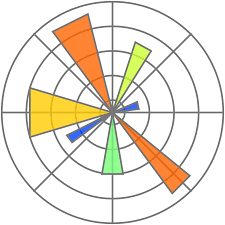
\includegraphics[scale=0.3]{matplotlib}
	\end{wrapfigure}
\textit{Matplotlib} è una libreria Python ampiamente utilizzata per la \textit{visualizzazione di dati e la creazione di grafici}. Fornisce un'interfaccia intuitiva per creare una vasta gamma di \textit{grafici}, inclusi \textit{grafici a linee}, \textit{grafici a dispersione}, \textit{istogrammi}, \textit{grafici a barre}, \textit{grafici a torta} e molti altri.

Permette di personalizzare svariati aspetti dei grafici, come colori, stili di linea, etichette degli assi e titoli.

Un punto di forza della libreria è la sua integrazione con NumPy, precedentemente introdotta. È possibile utilizzare gli array NumPy come dati di input per generare grafici, semplificando notevolmente il processo di visualizzazione dei dati.

In conclusione, Matplotlib è una potente libreria di visualizzazione dei dati in Python, la cui flessibilità, facilità d'uso e integrazione con NumPy la rendono uno strumento essenziale per gli scienziati, gli ingegneri e i data scientist.
\newpage
{\section{GIL e Multiprocessing}
	
	\begin{wrapfigure}{l}{0.20\textwidth}
		\centering
		
\includegraphics[scale=0.30]{multiprocessing}
	\end{wrapfigure}
Il \textit{GIL (Global Interpreter Lock)} è un meccanismo di gestione dei thread utilizzato nell'implementazione standard di CPython, l'interprete di Python di riferimento, allo scopo di consentire un'interazione più sicura con gli oggetti Python.

Il GIL è un \textit{vincolo} che permette a solo un thread alla volta di eseguire istruzioni Python, \textbf{anche su sistemi con processori multi-core}. Questo significa che, nonostante si possano utilizzare thread multipli, essi non possono eseguire istruzioni simultaneamente: quando un thread acquisisce il GIL, gli altri thread devono attendere il loro turno per eseguire codice Python.

Rappresenta un \textit{limite sulle prestazioni} in alcune situazioni specifiche, in particolare quando si tenta di applicare una parallelizzazione al fine di sfruttare appieno le capacità di elaborazione parallela di un sistema multi-core.

Il modulo \textit{multiprocessing}, incluso nelle librerie standard di Python, offre una soluzione per superare le limitazioni del GIL. Fornisce un'interfaccia per la \textit{creazione di processi multipli}, che possono eseguire codice Python \textbf{in modo indipendente} e sfruttare i vantaggi del parallelismo effettivo su sistemi multi-core.

Utilizzando multiprocessing, è possibile suddividere un compito in più processi che vengono essere eseguiti in parallelo. Tali processi comunicano tra loro attraverso la condivisione di dati o l'invio di messaggi tramite code o pipe.

Tuttavia, l'utilizzo di multiprocessing non è privo di svantaggi:
\begin{itemize}
	\item Se il lavoro da eseguire in ogni processo è relativamente semplice e richiede poco tempo di calcolo, il costo aggiuntivo di creare e gestire i processi potrebbe superare i benefici del parallelismo;
	\item Se i processi devono comunicare o dipendere l'uno dall'altro in modo significativo durante l'esecuzione, l'utilizzo di multiprocessing può introdurre complessità aggiuntiva;
	\item Ogni processo creato con multiprocessing ha il proprio spazio di memoria separato. Se il processo richiede una grande quantità di dati da elaborare e mantenere in memoria, l'utilizzo di processi multipli può portare a un consumo eccessivo di memoria;
	\item L'invio di dati tra processi richiede la \textit{serializzazione} e la \textit{deserializzazione} degli oggetti utilizzando \textit{pickle}. Questa conversione non supporta tutti i tipi di dati e introduce un certo overhead, soprattutto per oggetti complessi o di grandi dimensioni;
\end{itemize}
\chapter{MultiProcess Image Processing Bench}
\begin{figure}[H]
	\centering
	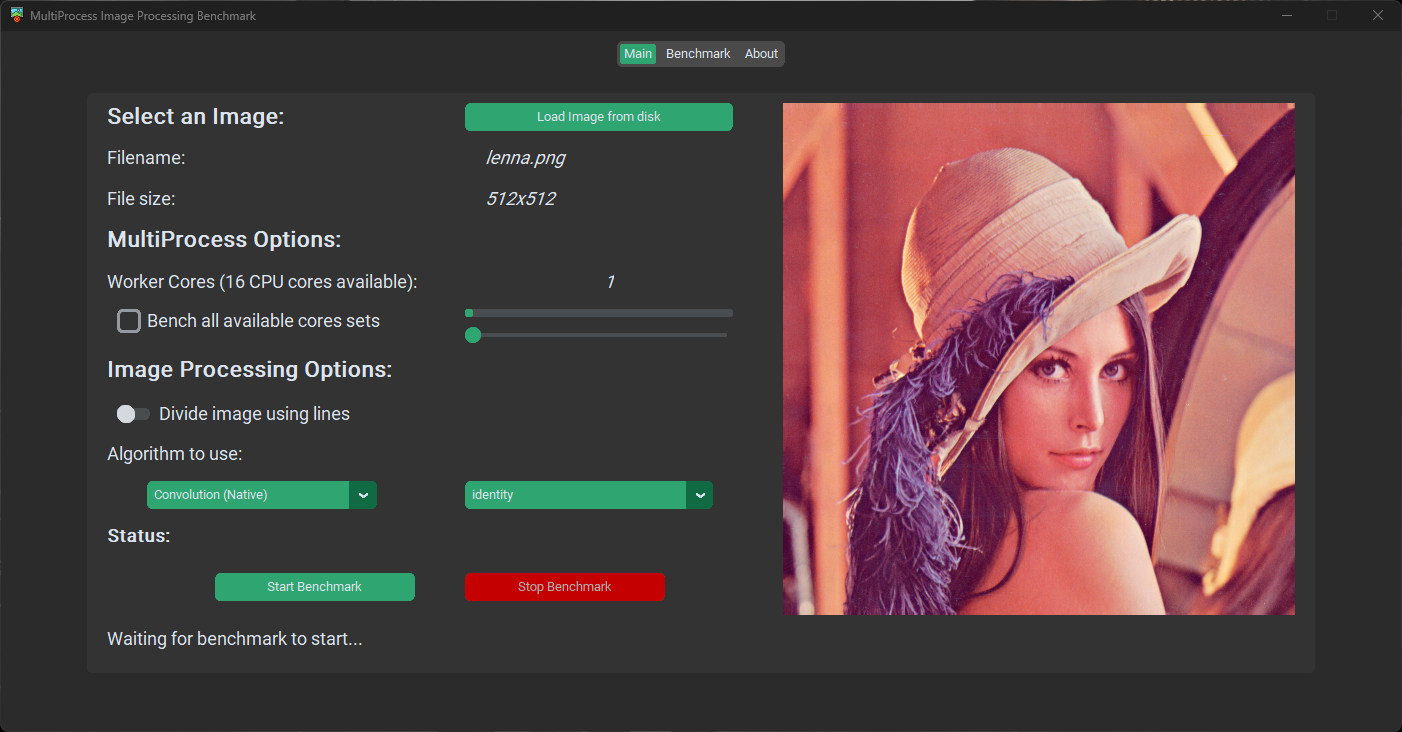
\includegraphics[width=\linewidth]{main-window}
	\caption{Schermata principale dell'applicativo}
\end{figure}
L'applicativo software sviluppato è denominato \textit{"MultiProcess Image Processing Bench"}, a cui, per semplicità, sarà fatto riferimento tramite l'abbreviazione \textit{"Benchmarker"}.\\
\newline
\textit{Benchmarker} è un programma dotato di interfaccia grafica sviluppato in Python 3 con Tkinter, e quindi supportato su MacOS, Linux e Windows. L'applicativo prende in input un'immagine di dimensioni quadrate, ridimensionandola se necessario, esegue un algoritmo di image processing secondo una configurazione utente e restituisce i tempi di esecuzione sotto forma di grafico a barre laterali.\par
Lo scopo di \textit{Benchmarker} è rendere facile ed automatico il confronto delle prestazioni di un certo algoritmo di image processing eseguito su diverse configurazioni di parallelismo.

\section{Uso del programma}
Benchmarker fa uso di librerie esterne, come ad esempio \textit{pillow} e \textit{matplotlib}. Per questo motivo, prima di poter utilizzare il programma è necessario installare tramite \textit{"pip"}, il package installer di Python, le dipendenze in uno dei seguenti modi:
\begin{itemize}
	\item \textit{Global Package}: installare le dipendenze direttamente nel sistema, diventando di fatto globali e accessibili da qualunque script Python eseguito nel sistema;
	\item \textit{Virtual Environment}: creare un ambiente virtuale in cui installare le dipendenze;
\end{itemize}
Una volta installate le dipendenze, per utilizzare Benchmarker, e quindi visualizzare l'interfaccia grafica, è necessario avviare lo script \textit{main.py}.

Una volta aperto il programma è possibile:
\begin{enumerate}
	\item caricare l'immagine su cui eseguire gli algoritmi, qualora l'immagine non fosse di \textit{dimensioni quadrate} verrà chiesto di ridimensionarla;
	\item scegliere il \textit{quantitativo di core} da utilizzare per l'\textit{esecuzione parallela}, il \textit{numero totale di core} dipende dal processore del calcolatore in cui si sta eseguendo l'applicativo;
	\item selezionare la \textit{modalità di suddivisione} in \textbf{linee o quadrati} dell'immagine originale, qualora si scelga la suddivisione in quadrati, il quantitativo di core dovrà essere un \textit{quadrato perfetto};
	\item scegliere se provare o meno tutte le possibili configurazioni parallelo eseguibili nel calcolatore;
	\item selezionare la \textit{tipologia di algoritmo}, ed eventualmente l'algoritmo specifico, inserendo, se richiesti, i parametri dello stesso;
	\item \textit{avviare il benchmark};
\end{enumerate}	
\noindent
Una volta avviato il benchmark, verrà prima eseguita un'\textit{esecuzione sequenziale} dell'algoritmo e successivamente la/le \textit{configurazioni parallele} scelte dall'utente. I risultati verranno visualizzati nell'apposita finestra.
 \begin{figure}[H]
 	\centering
 	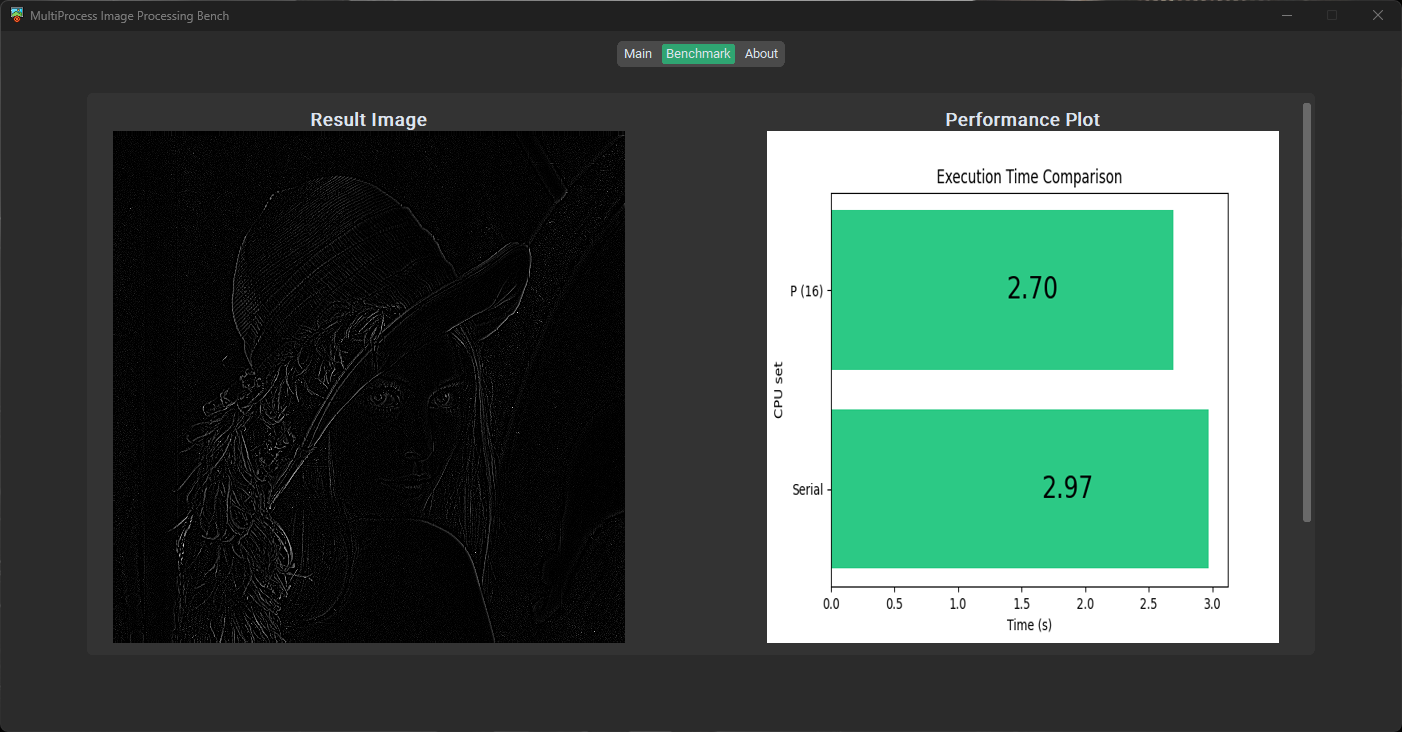
\includegraphics[width=\linewidth]{bench-results}
 	\caption{Esempio di risultati del benchmark}
 \end{figure}

\section{Suddivisione dell'immagine}
Alla base del parallelismo vi è il concetto di \textit{suddividere un grande problema in sotto problemi più piccoli della stessa natura}.
Per quanto riguarda l'image processing tale concetto viene applicato suddividendo un'immagine in \textit{sotto immagini}, ovvero immagini che se riunite ricostruiscono l'immagine originale.
Per tale operazione Benchmarker mette a disposizione due modalità:
\begin{itemize}
	\item \textit{Suddivisione in strisce, o linee}: l'immagine originale viene suddivide in $N$ linee quanti sono i core selezionati per l'esecuzione parallela, ogni processo parallelo eseguirà l'algoritmo sull'immagine parziale assegnatogli e restituirà il risultato parziale, che verrà unito agli altri per formare il risultato completo;
	\begin{itemize}
		\item la \textit{lunghezza della striscia} viene calcolata semplicemente dividendo il lato del quadrato per $N$, numero di linee;
	\end{itemize}
	\item \textit{Suddivisione in quadrati}: l'immagine originale viene suddivide in $M = \sqrt{N}$ quadrati, dove $N$ è il numero di core selezionati per l'esecuzione parallela, ogni processo parallelo eseguirà l'algoritmo sull'immagine parziale assegnatogli e restituirà il risultato parziale, che verrà unito agli altri per formare il risultato completo;
	\begin{itemize}
		\item la \textit{lunghezza del quadrato} viene calcolata semplicemente dividendo il lato del quadrato per $M$, numero di quadrati;
		\item il \textit{numero di core} selezionato per l'esecuzione parallela deve essere un \textit{quadrato perfetto};
	\end{itemize}
\end{itemize}
\noindent La logica per la suddivisione implementata in Python è presente in appendice: \ref{appendix:lines_subdivision}.
 \begin{figure}[H]
	\centering
	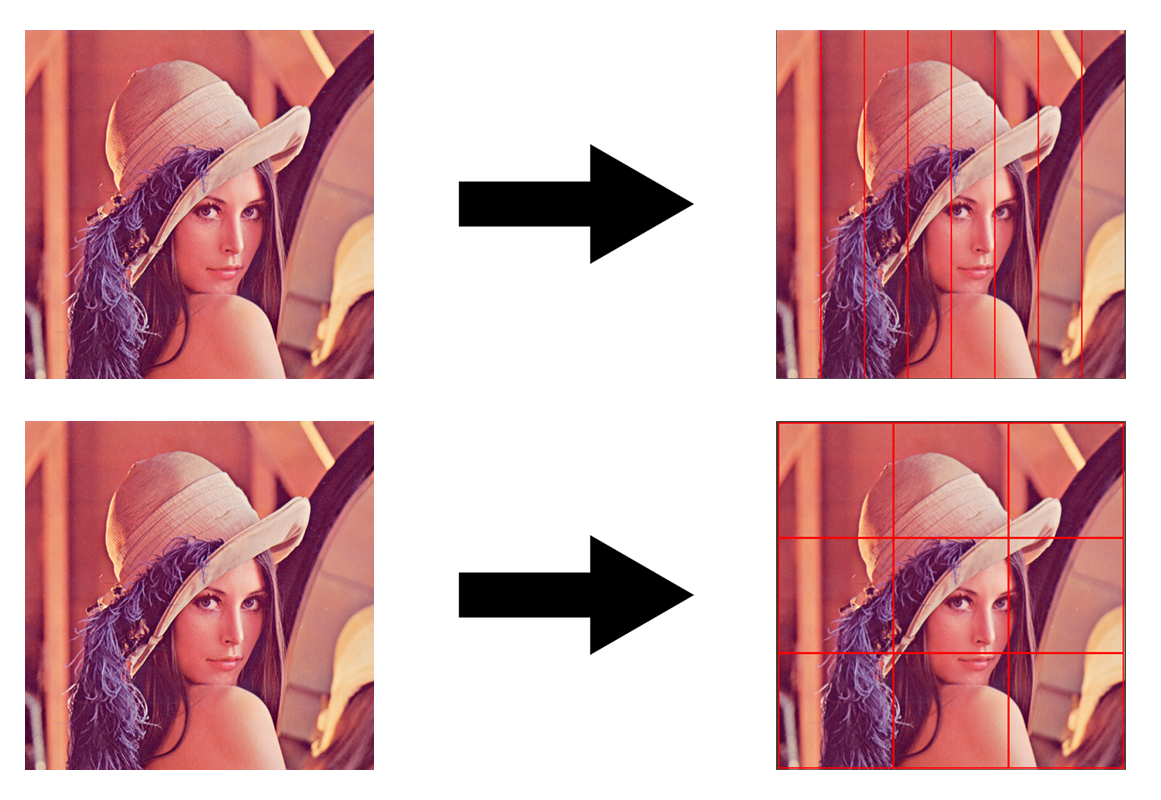
\includegraphics[width=\linewidth]{sub-images-preview}
	\caption{Esempio di suddivisione}
\end{figure}

\section{Algoritmi implementati}
All'interno di Benchmarker sono stati implementati alcuni dei più famosi algoritmi dell'image processing.

Per \textit{scelta di stile e coerenza dei risultati}, tali algoritmi, come convoluzione e operatori morfologici, sono \textit{implementati facendo uso delle funzionalità native di Python} senza l'utilizzo delle funzioni avanzate offerte dalle librerie, in quanto implementate con un riguardo alle prestazioni in C.
\newpage

\subsection{Convoluzione}
La \textit{convoluzione} è un'operazione fondamentale nell'elaborazione delle immagini utilizzata per analizzare e modificare le caratteristiche di un'immagine. In sintesi, la convoluzione consiste nel sovrapporre un \textit{kernel} su un'immagine e calcolare la somma dei prodotti degli elementi sovrapposti del kernel e dei pixel corrispondenti dell'immagine.

Il \textit{kernel} è una piccola matrice di valori numerici, di \textit{dimensioni generalmente dispari}, che definisce come combinare i pixel circostanti durante l'operazione di convoluzione. Ogni elemento del kernel viene moltiplicato con il valore corrispondente del pixel nell'immagine, e i risultati vengono sommati per ottenere il valore convoluto per il pixel centrale.

Questo processo viene ripetuto per ogni pixel dell'immagine.

 \begin{figure}[H]
	\centering
	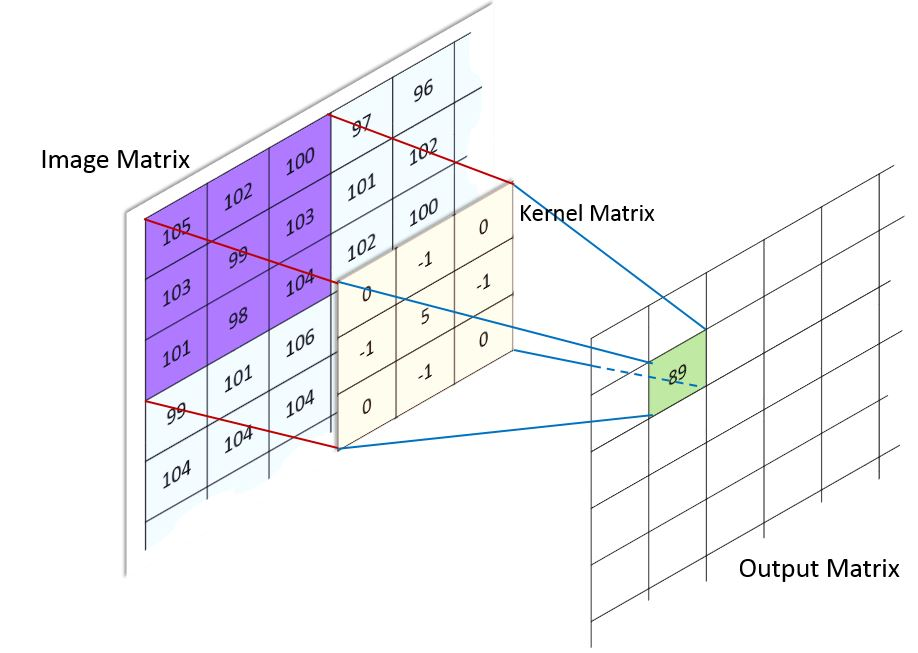
\includegraphics[scale=0.5]{conv-matrix}
	\caption{Schema della convoluzione}
\end{figure}

\noindent La convoluzione viene spesso utilizzata per applicare filtri e operazioni di modifica dell'immagine che richiedono kernel specifici, ideati per ottenere un determinato effetto.

La logica della convoluzione implementata in Python è presente in appendice: \ref{appendix:convolution}

\subsubsection{Identity}
Il kernel \textit{Identity} rappresenta il più semplice filtro convolutivo: non effettua alcuna modifica all'immagine di input.\newline
\begin{equation*}
	\text {Identity Kernel} = 
	\begin{bmatrix}
		0 & 0 & 0 \\
		0 & 1 & 0 \\
		0 & 0 & 0
	\end{bmatrix}
\end{equation*}
\newline Quando viene applicato a un'immagine tramite la convoluzione, mantiene inalterati i valori dei pixel. Ciò significa che il pixel di output nella posizione corrispondente al pixel di input sarà uguale al valore del pixel di input stesso. In pratica, l'immagine convoluta con il kernel identità sarà identica all'immagine di input.
 \begin{figure}[H]
	\centering
	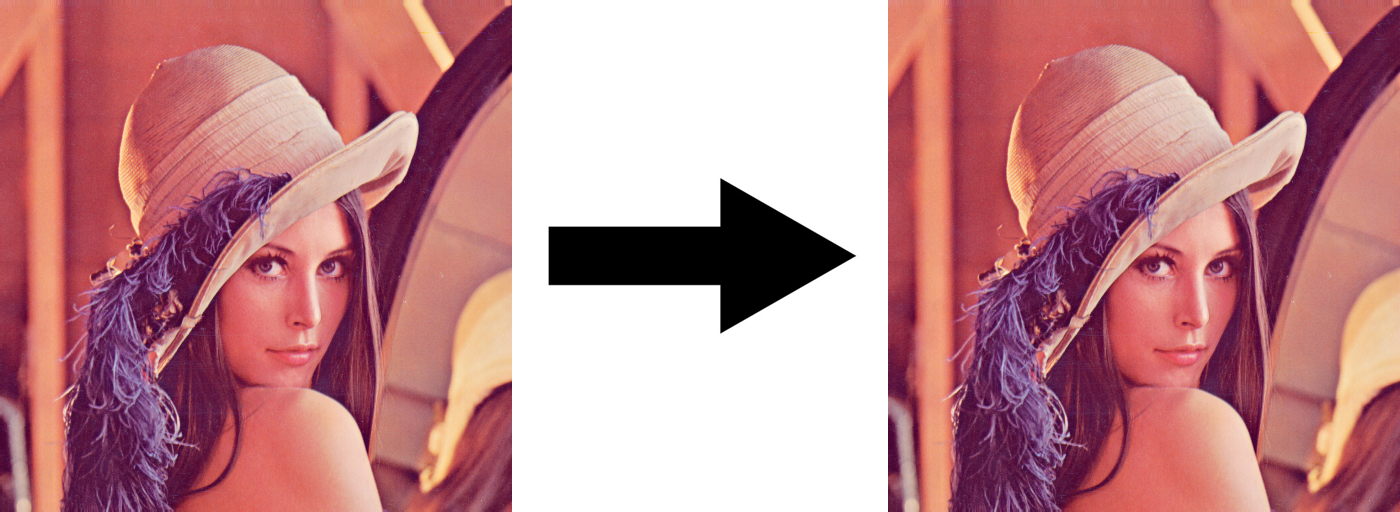
\includegraphics[width=\linewidth]{identity}
	\caption{Esempio di Kernel Identity}
\end{figure}
\subsubsection{Sobel-X e Sobel-Y}
I kernel di \textit{Sobel-X} e \textit{Sobel-Y} sono utilizzati per il rilevamento dei bordi. In particolare, \textit{Sobel-X} evidenzia i cambiamenti di intensità orizzontali, mentre \textit{Sobel-Y} quelli verticali.\newline
\begin{equation*}
	\text {Sobel-X} = 
	\begin{bmatrix}
		-1 & 0 & 1 \\
		-2 & 1 & 2 \\
		-1 & 0 & 1
	\end{bmatrix},
	\quad
	\text {Sobel-Y} = 
	\begin{bmatrix}
		-1 & -2 & -1 \\
		0 & 0 & 0 \\
		1 & 2 & 1
	\end{bmatrix},
\end{equation*}
\newline Quando vengono applicati a un'immagine tramite la convoluzione, calcolano le derivate parziali rispetto alle direzioni orizzontali e verticali, rispettivamente. Questo significa rilevano le variazioni di intensità lungo le linee orizzontali e verticali dell'immagine.
\begin{figure}[H]
	\centering
	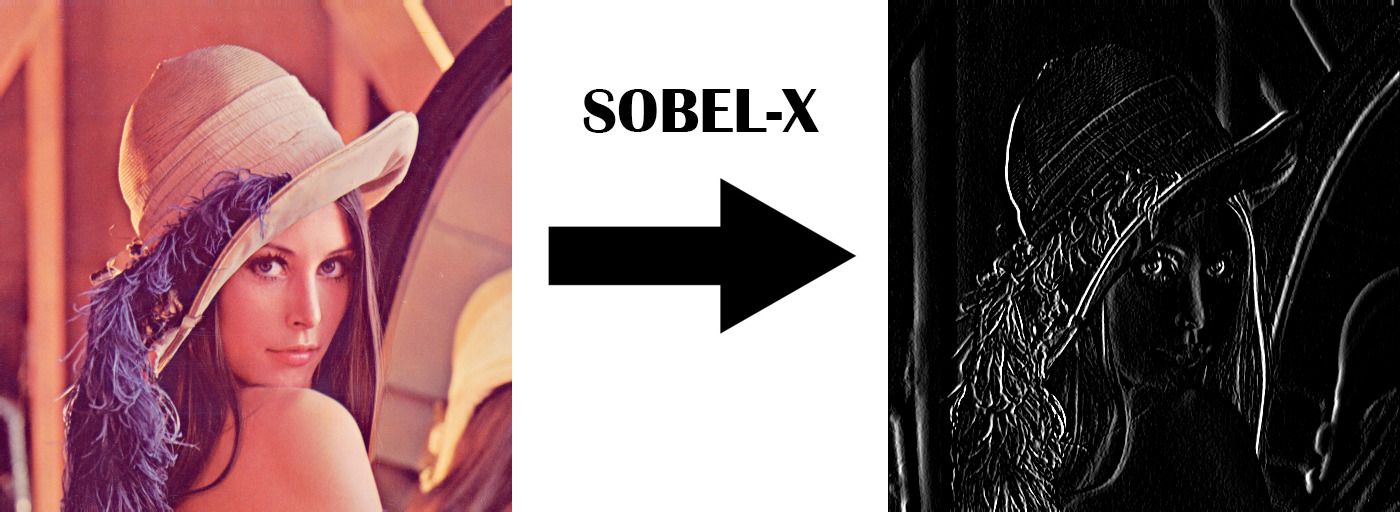
\includegraphics[width=\linewidth]{sobel-x}
	\caption{Esempio di Kernel Sobel-X}
\end{figure}
\begin{figure}[H]
	\centering
	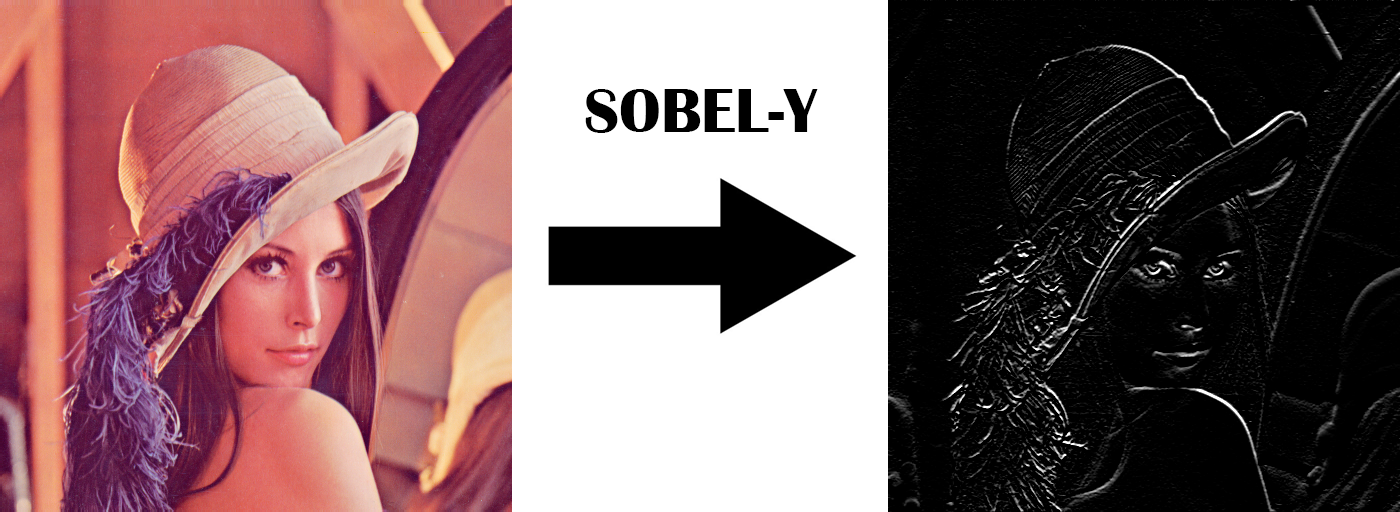
\includegraphics[width=\linewidth]{sobel-y}
	\caption{Esempio di Kernel Sobel-Y}
\end{figure}
\subsubsection{Prewitt-X e Prewitt-Y}
Simili ai kernel Sobel, i kernel di \textit{Prewitt-X} e \textit{Prewitt-Y} sono utilizzati per il rilevamento dei bordi. In particolare, \textit{Prewitt-X} evidenzia i cambiamenti di intensità orizzontali, mentre \textit{Prewitt-Y} quelli verticali.\newline
\begin{equation*}
	\text {Prewitt-X} = 
	\begin{bmatrix}
		-1 & 0 & 1 \\
		-1 & 0 & 1 \\
		-1 & 0 & 1
	\end{bmatrix},
	\quad
	\text {Prewitt-Y} = 
	\begin{bmatrix}
		-1 & -1 & -1 \\
		0 & 0 & 0 \\
		1 & 1 & 1
	\end{bmatrix},
\end{equation*}
\newline Quando vengono applicati a un'immagine tramite la convoluzione, calcolano le derivate parziali rispetto alle direzioni orizzontali e verticali, rispettivamente. Questo significa rilevano le variazioni di intensità lungo le linee orizzontali e verticali dell'immagine.

Rispetto ai kernel Sobel, producono un immanine meno nitida.
\begin{figure}[H]
	\centering
	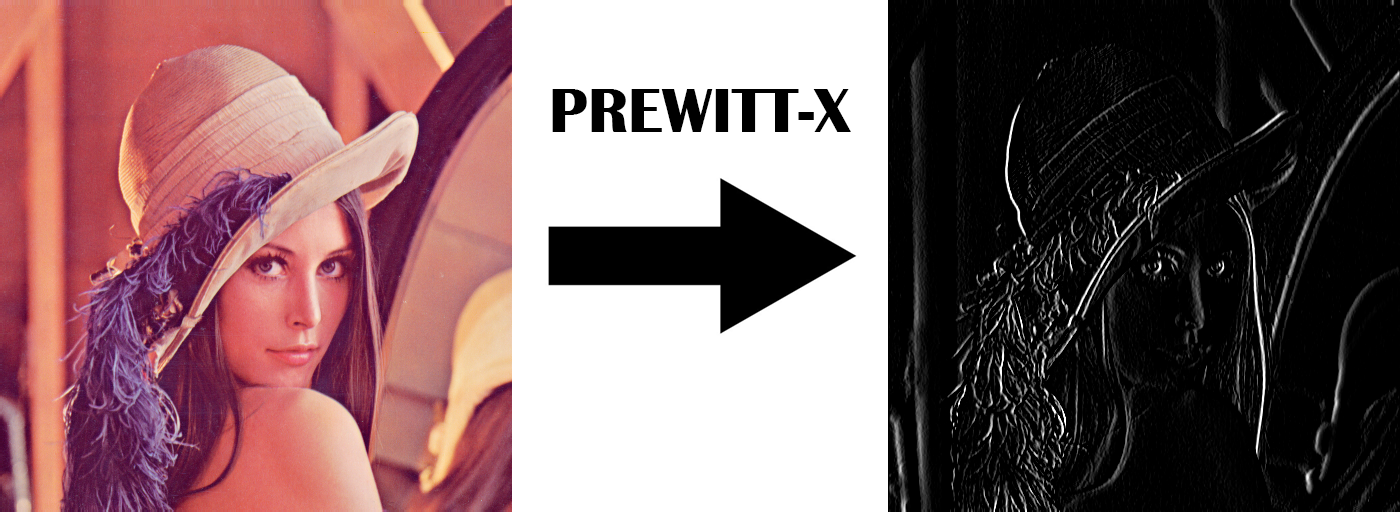
\includegraphics[width=\linewidth]{prewitt-x}
	\caption{Esempio di Kernel Prewitt-X}
\end{figure}
\begin{figure}[H]
	\centering
	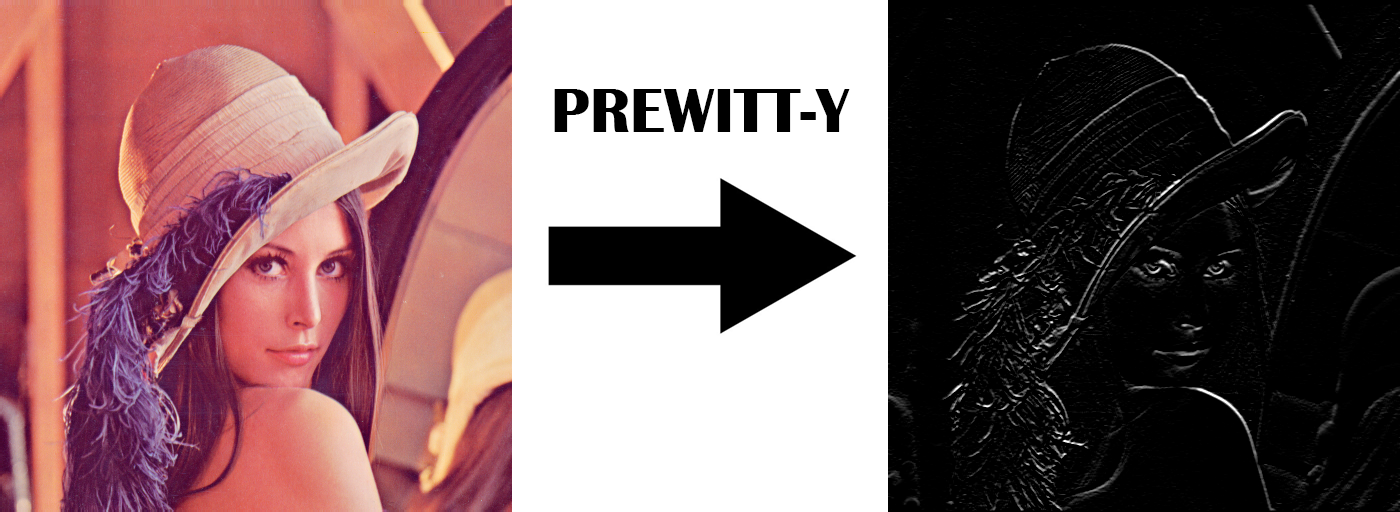
\includegraphics[width=\linewidth]{prewitt-y}
	\caption{Esempio di Kernel Prewitt-Y}
\end{figure}
\subsubsection{Laplacian}
Il kernel di \textit{Laplacian} è utilizzato per il rilevamento dei bordi o dei punti di discontinuità.\newline
\begin{equation*}
	\text {Laplacian} = 
	\begin{bmatrix}
		0 & -1 & 0 \\
		-1 & 4 & -1 \\
		0 & -1 & 0
	\end{bmatrix}
\end{equation*}
\newline Quando viene applicato a un'immagine tramite la convoluzione, produce una mappa dei gradienti del secondo ordine, che rappresenta la variazione dell'intensità dei pixel nell'immagine, generando un'immagine convoluta che evidenzia i bordi, le linee e altre caratteristiche forti dell'immagine.

Tuttavia, può anche produrre una risposta forte al rumore presente nell'immagine, poiché amplifica le variazioni di intensità in tutte le direzioni.
\begin{figure}[H]
	\centering
	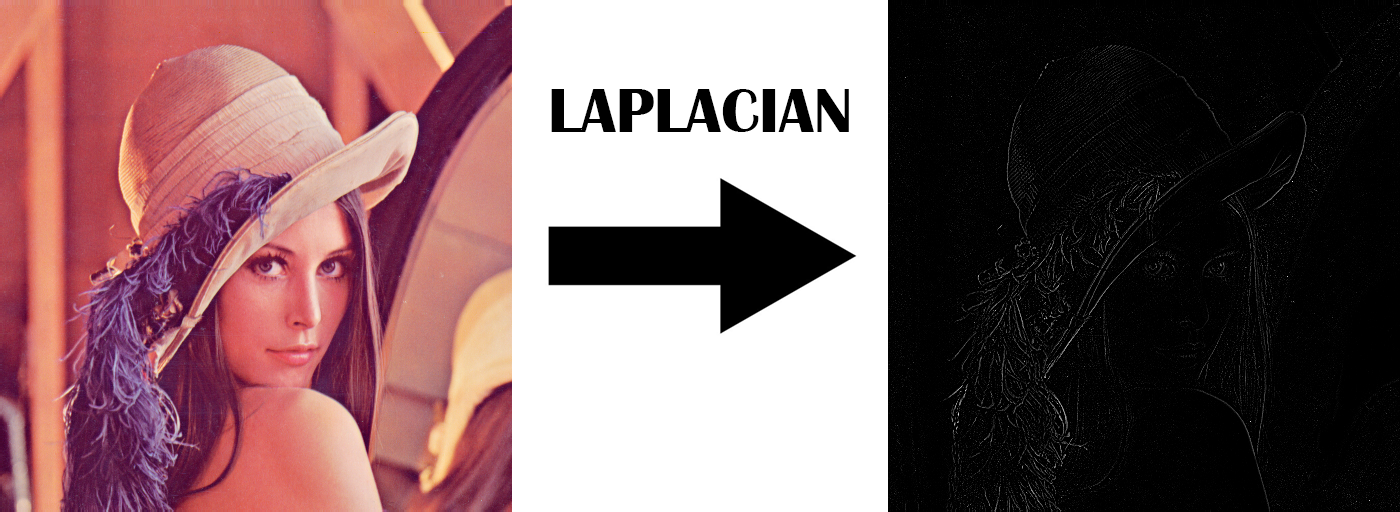
\includegraphics[width=\linewidth]{laplacian}
	\caption{Esempio di Kernel Laplacian}
\end{figure}
\subsubsection{Sharpen e High-Pass}
I kernel di \textit{Sharpen} e \textit{High-Pass} sono utilizzati per enfatizzare le componenti ad alta frequenza e attenuare quelle a bassa frequenza producendo un miglioramento dei dettagli di un'immagine.\newline
\begin{equation*}
	\text {Sharpen} = 
	\begin{bmatrix}
		0 & -1 & 0 \\
		-1 & 5 & -1 \\
		0 & -1 & 0
	\end{bmatrix},
	\quad
	\text {High-Pass} = 
	\begin{bmatrix}
		0 & -1/4 & 0 \\
		-1/4 & 2 & -1/4 \\
		0 & -1/4 & 0
	\end{bmatrix}
\end{equation*}
\newline Quando vengono applicati a un'immagine tramite la convoluzione, producono un'immagine convoluta in cui i bordi e i dettagli sono enfatizzati, migliorando il contrasto tra i pixel adiacenti e accentuando le transizioni di intensità.

Questo può portare ad un aspetto più definito e nitido dell'immagine.
\begin{figure}[H]
	\centering
	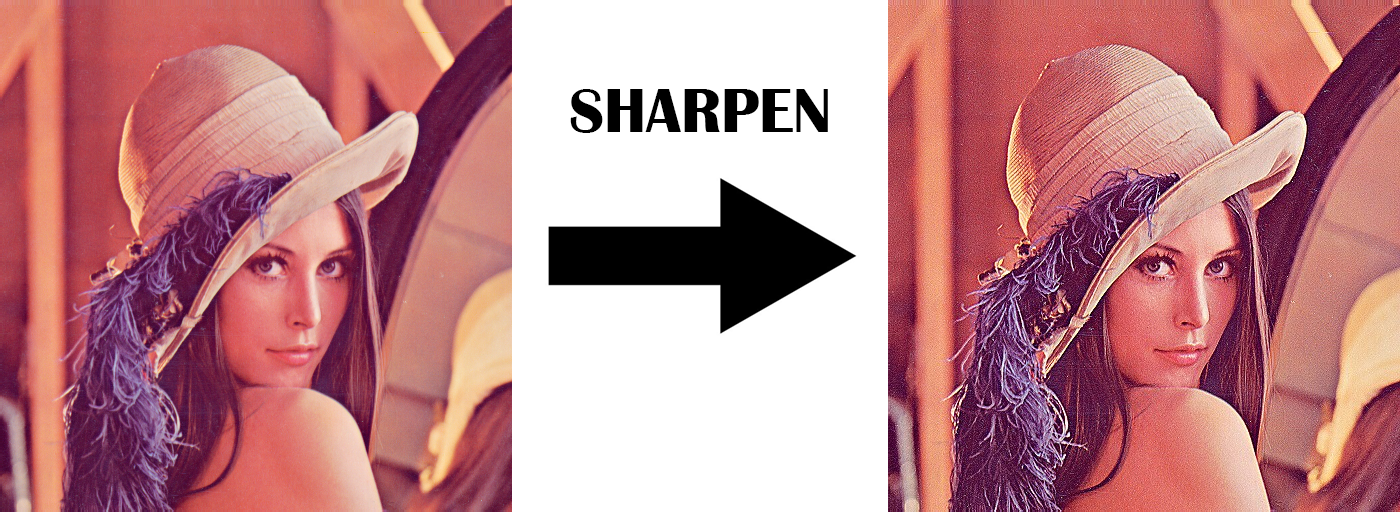
\includegraphics[width=\linewidth]{sharpen}
	\caption{Esempio di Kernel Sharpen}
\end{figure}
\begin{figure}[H]
	\centering
	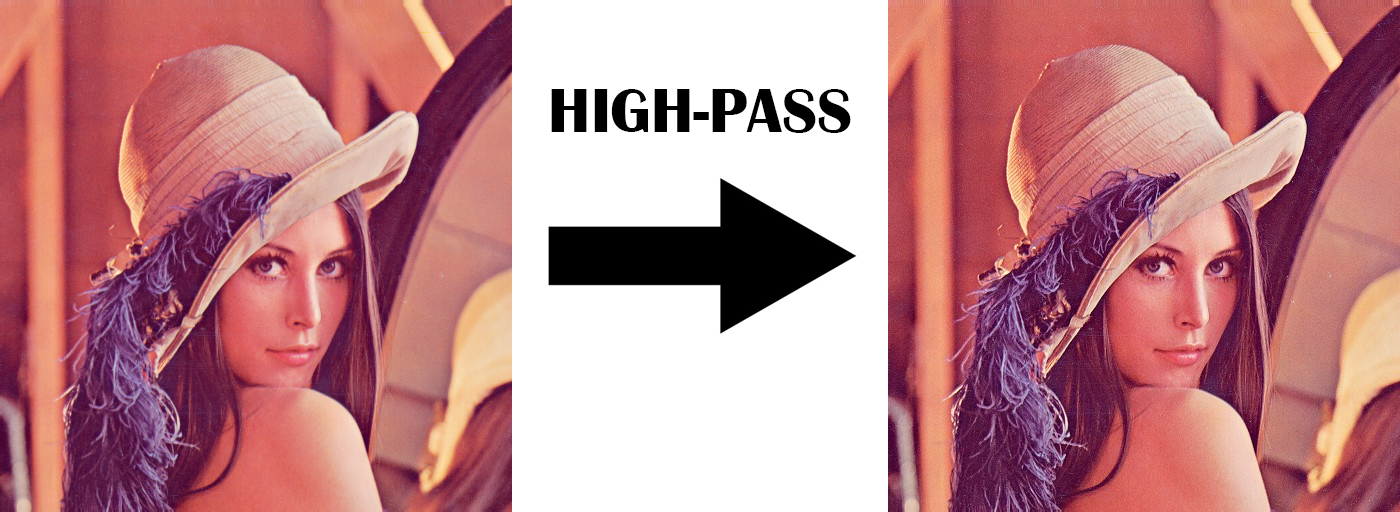
\includegraphics[width=\linewidth]{high-pass}
	\caption{Esempio di Kernel High-Pass}
\end{figure}
\subsubsection{Blur (Low-Pass)}
Il kernel di \textit{Low-Pass} è utilizzato per attenuare le componenti ad alta frequenza e mantiene le componenti a bassa frequenza, consentendo di eliminare il rumore e ottenere un'immagine più morbida.\newline
\begin{equation*}
	\text {Low-Pass} = 
	\begin{bmatrix}
		1/9 & 1/9 & 1/9 \\
		1/9 & 1/9 & 1/9 \\
		1/9 & 1/9 & 1/9
	\end{bmatrix}
\end{equation*}
\newline Quando viene applicato a un'immagine tramite la convoluzione, produce un'immagine convoluta in cui le transizioni brusche dell'intensità vengono attenuate e l'immagine risulta più sfocata.
\begin{figure}[H]
	\centering
	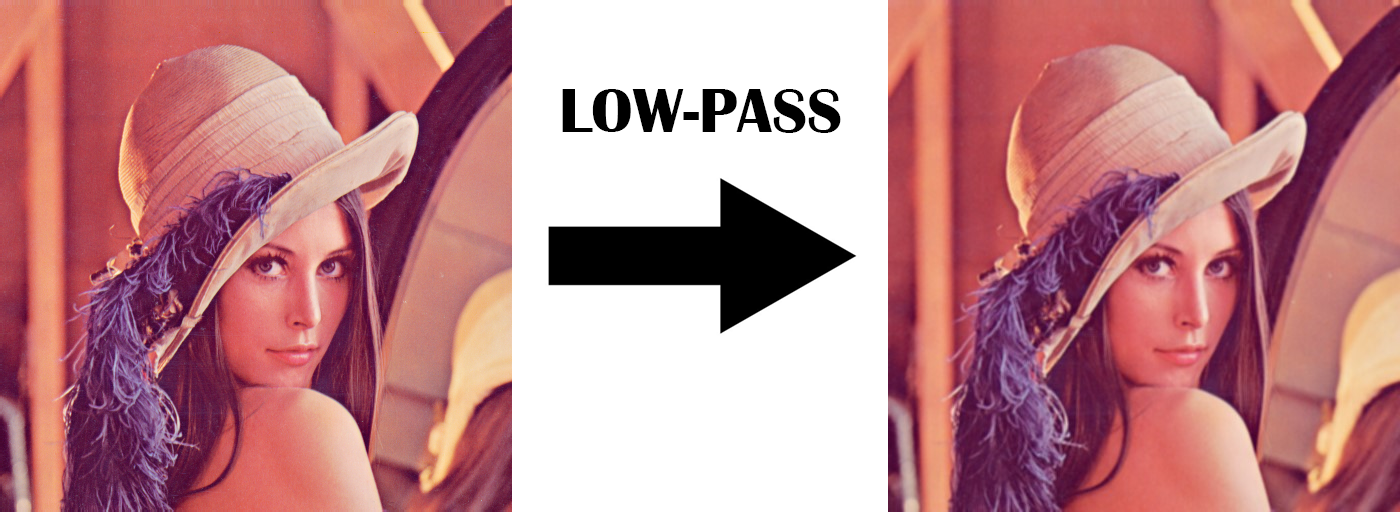
\includegraphics[width=\linewidth]{low-pass}
	\caption{Esempio di Kernel Low-Pass}
\end{figure}

\subsubsection{Blur (Gaussian)}
Il kernel di \textit{Gaussian} è utilizzato per eseguire una riduzione del rumore e una sfocatura dell'immagine\newline
\begin{equation*}
	\text {Gaussian 3x3} = 
	\begin{bmatrix}
		1/16 & 2/16 & 1/16 \\
		2/16 & 4/16 & 2/16 \\
		1/16 & 2/16 & 1/16
	\end{bmatrix}
\end{equation*}
\newline Quando viene applicato a un'immagine tramite la convoluzione, produce un effetto di sfocatura, riducendo le variazioni di intensità tra i pixel e attenuando il rumore ad alta frequenza.

L'uso del kernel gaussiano permette di ottenere una sfocatura più naturale e graduale rispetto ad altri filtri di sfocatura più semplici, poiché tiene conto delle distribuzioni di intensità circostanti, rendendo la transizione da un pixel all'altro più morbida e realistica.

Fornendo una dimensione e un valore sigma, Benchmarker può generare un kernel di Gaussian che rispetti i parametri forniti.

La logica per la generazione di un kernel gaussiano di una certa \textit{dimensione} con un certo \textit{sigma} implementata in Python è presente in appendice: \ref{appendix:gauss}
\begin{figure}[H]
	\centering
	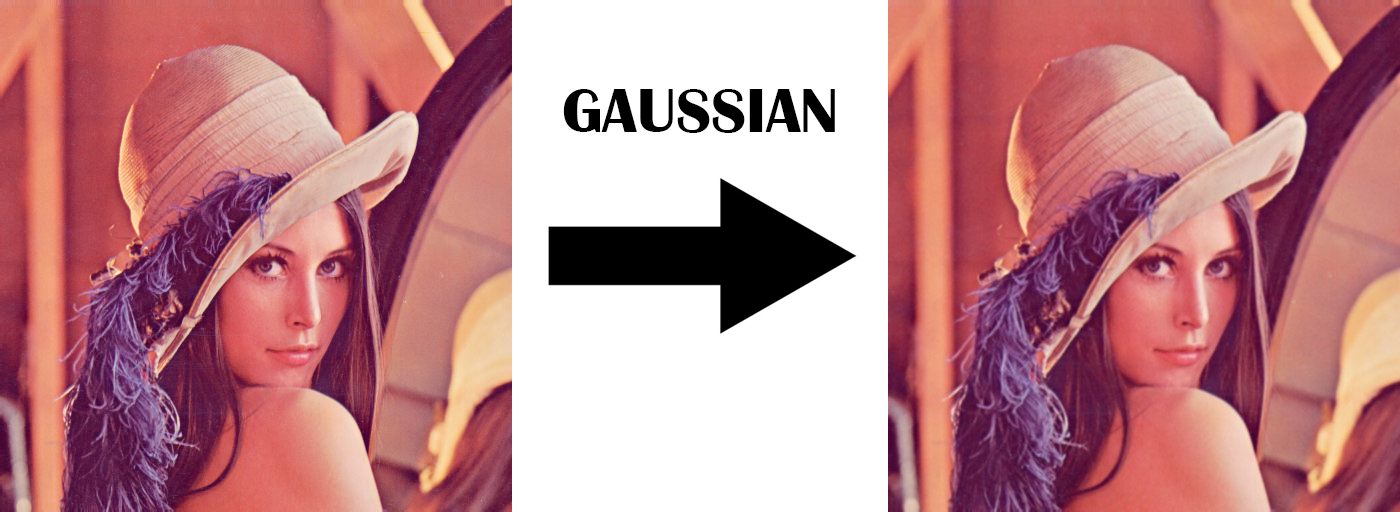
\includegraphics[width=\linewidth]{gaussian}
	\caption{Esempio di Kernel Gaussian}
\end{figure}

\subsection{Operatori Morfologici}
Gli \textit{operatori morfologici} sono utilizzati per manipolare la forma, la struttura e le caratteristiche di un'immagine. Queste operazioni si basano su principi matematici che coinvolgono l'interazione tra un \textit{elemento strutturante} e i pixel dell'immagine.

Gli \textit{elementi strutturanti}, anche chiamati \textit{kernel di forma}, sono matrici che definiscono la forma e la dimensione dell'area circostante a ciascun pixel durante l'applicazione degli operatori morfologici. \textit{Questi elementi strutturanti svolgono un ruolo cruciale nel determinare l'effetto dell'operazione morfologica sull'immagine}.\newline\newline
\noindent\textit{Benchmarker} implementa e permette la selezione dei seguenti elementi strutturali:
\begin{equation*}
	\text {Square} = 
	\begin{bmatrix}
		1 & 1 & 1\\
		1 & 1 & 1\\
		1 & 1 & 1
	\end{bmatrix}
	\text {Cross} = 
	\begin{bmatrix}
		0 & 1 & 0\\
		1 & 1 & 1\\
		0 & 1 & 0
	\end{bmatrix}
	\text {Line} = 
	\begin{bmatrix}
		0 & 0 & 0\\
		1 & 1 & 1\\
		0 & 0 & 0
	\end{bmatrix}
	\text {Circle} = 
	\begin{bmatrix}
		0 & 1 & 1 & 1 & 0\\
		1 & 1 & 1 & 1 & 1\\
		1 & 1 & 1 & 1 & 1\\
		1 & 1 & 1 & 1 & 1\\
		0 & 1 & 1 & 1 & 0
	\end{bmatrix}
\end{equation*}

\noindent \textit{Benchmarker} implementa gli operatori morfologici di erosione e dilatazione, i cui codici sono presenti in appendice: \ref{appendix:erosion}.

\subsubsection{Erosione}
L'erosione è un'operazione morfologica che riduce le regioni o i dettagli di un'immagine. Durante l'erosione, ogni pixel nell'immagine viene confrontato con il corrispondente sotto l'elemento strutturante. Se tutti i pixel sottostanti l'elemento strutturante sono \textit{attivi}, cioè hanno un valore di intensità alto, il pixel corrispondente nell'immagine risultante viene mantenuto attivo. In caso contrario, il pixel viene disattivato o eliminato. L'erosione tende a ridurre la dimensione degli oggetti e a rimuovere piccoli dettagli, consentendo di separare le regioni connesse.

\begin{figure}[H]
	\centering
	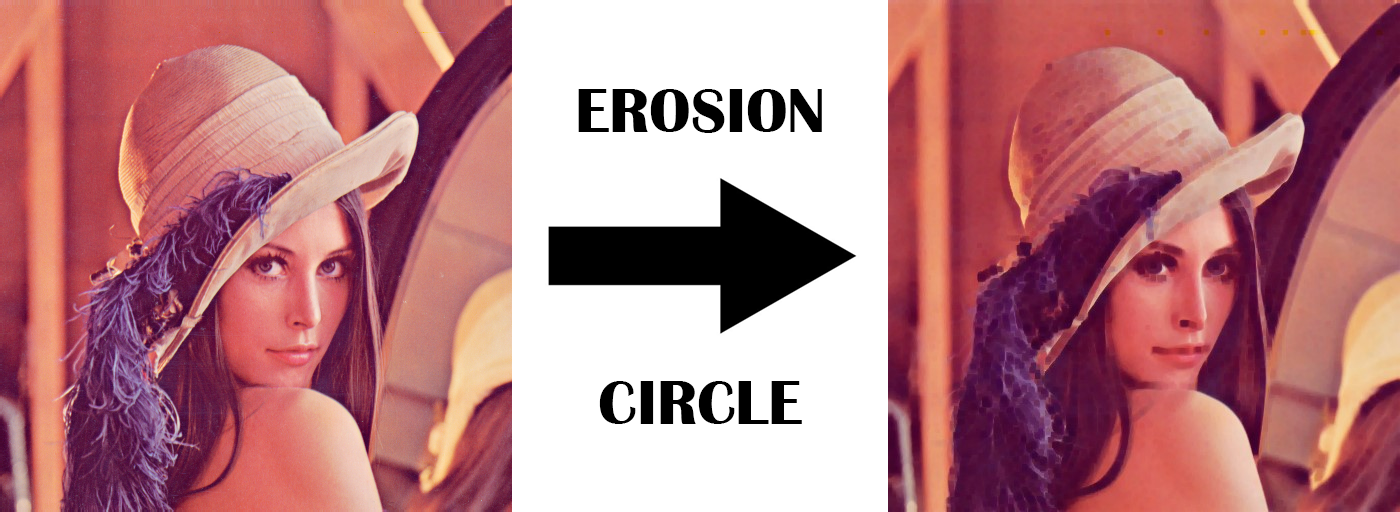
\includegraphics[width=\linewidth]{erosion}
	\caption{Esempio Erosione con elemento strutturante Circle}
\end{figure}

\subsubsection{Dilatazione}
La dilatazione è un'altra operazione morfologica che ha l'effetto opposto dell'erosione. Durante la dilatazione, ogni pixel nell'immagine viene confrontato con il corrispondente sotto l'elemento strutturante. Se almeno un pixel sottostante l'elemento strutturante è \textit{attivo}, il pixel corrispondente nell'immagine risultante viene attivato o mantenuto attivo. La dilatazione tende ad espandere le regioni e a unire gli oggetti vicini.


\begin{figure}[H]
	\centering
	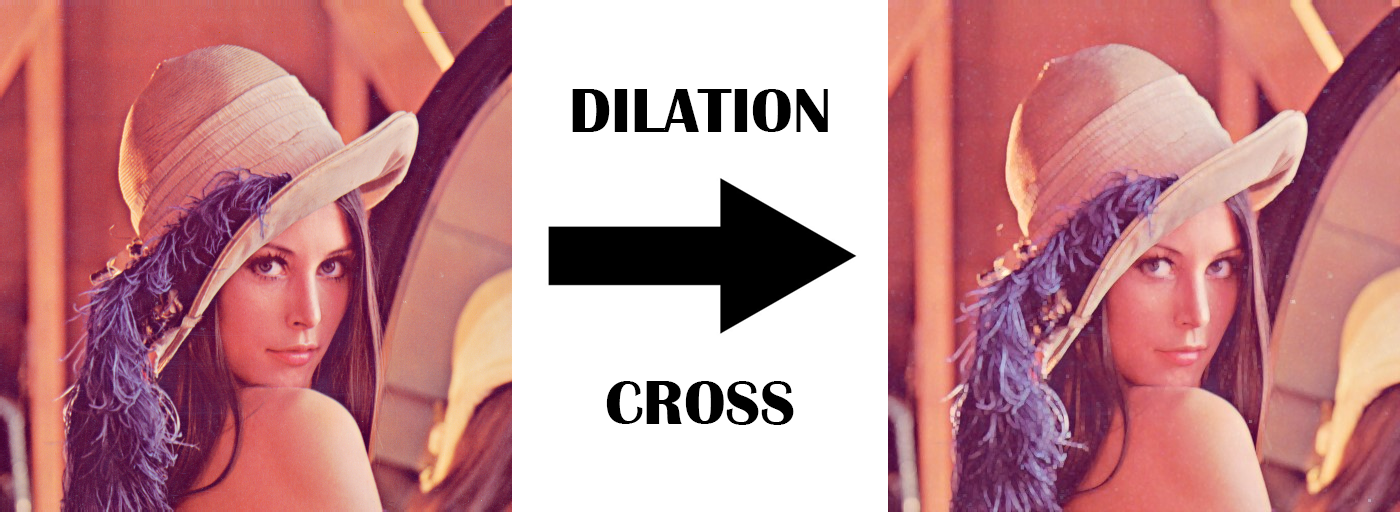
\includegraphics[width=\linewidth]{dilation}
	\caption{Esempio Dilatazione con elemento strutturante Cross}
\end{figure}

\subsection{Filtri di Noise Reduction}
I filtri di \textit{noise reduction}, o \textit{filtri di riduzione del rumore}, sono utilizzati per mitigare o eliminare il rumore presente nelle immagini digitali. Il rumore può essere causato da vari fattori, come le imperfezioni del sensore, le interferenze elettriche o il processo di acquisizione dell'immagine.

L'obiettivo principale è quello di migliorare la qualità dell'immagine, rimuovendo o riducendo il rumore senza influire eccessivamente sulla nitidezza e sui dettagli importanti dell'immagine.

\textit{Benchmarker} implementa il \textit{mean filter} e il \textit{bilateral} filter, , i cui codici sono presenti in appendice: \ref{appendix:mean}.

\subsubsection{Mean Filter}
Il \textit{filtro di media}, detto anche \textit{mean filter}, è uno dei filtri di noise reduction più semplici ed efficaci. Sostituisce il valore di ciascun pixel nell'immagine con la media dei valori dei pixel nell'intorno del pixel stesso.

In pratica, il filtro di media calcola la media aritmetica dei valori dei pixel all'interno di una finestra quadrata e sostituisce il valore del pixel corrente con questa media.

Questo processo aiuta a ridurre il rumore, poiché il rumore casuale tende ad avere un effetto minore sulla media dei valori dei pixel.

La dimensione dell'intorno viene decisa dall'utente al momento della selezione del filtro di media.

\begin{figure}[H]
	\centering
	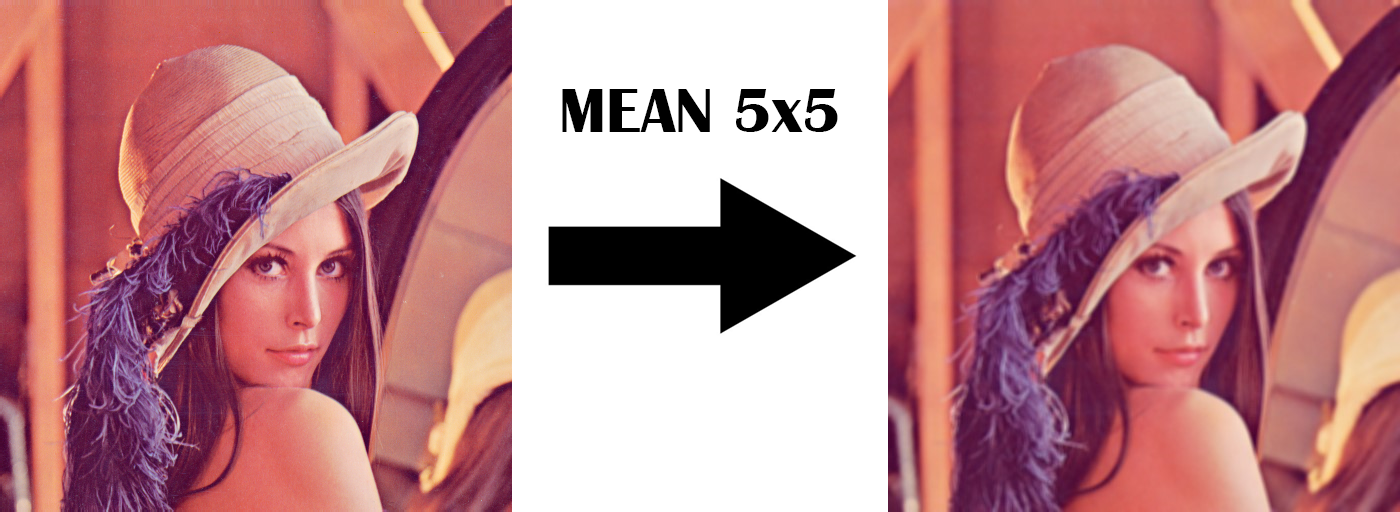
\includegraphics[width=\linewidth]{mean}
	\caption{Esempio di filtro di media 5x5}
\end{figure}

\subsubsection{Bilateral Filter}
Il \textit{filtro bilaterale}, detto anche \textit{bilateral filter} offre una maggiore flessibilità nel mantenere i confini e i dettagli dell'immagine. 

A differenza del filtro di media, il filtro bilaterale considera non solo i valori dei pixel nell'intorno, ma anche le differenze di intensità tra i pixel.

Questo filtro calcola una media ponderata dei valori dei pixel all'interno di una finestra, in base alla distanza spaziale tra i pixel e alla differenza di intensità tra i pixel.

Ciò significa che i pixel che sono simili in termini di intensità e vicini spazialmente avranno un peso maggiore nella media ponderata, mentre i pixel con differenze significative di intensità avranno un peso minore. In questo modo, il filtro bilaterale può ridurre il rumore, preservando al contempo i dettagli e i confini dell'immagine.

La dimensione dell'intorno, distanza spaziale e la differenza d'intensità vengono decisi dall'utente al momento della selezione del filtro bilaterale.

\begin{figure}[H]
	\centering
	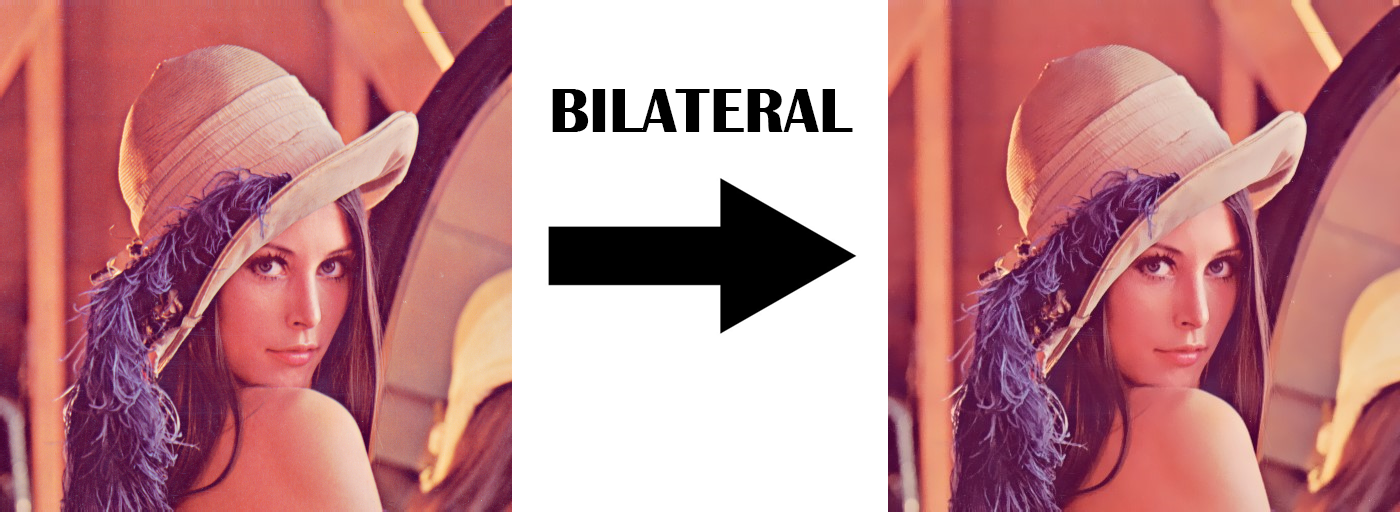
\includegraphics[width=\linewidth]{bilateral}
	\caption{Esempio di filtro bilaterale}
\end{figure}

\subsection{Canny}
Il \textit{filtro di Canny}, chiamato anche \textit{algoritmo di Canny}, è un popolare filtro di \textit{edge detection}. È un algoritmo composto da più passaggi che combinati insieme forniscono una buona precisione nel rilevamento dei bordi, riducendo al contempo il rumore.

L'algoritmo di Canny opera secondo i seguenti passaggi:
\begin{itemize}
	\item \textit{Riduzione del rumore}: l'immagine di input viene filtrata per ridurre il rumore. Viene applico un filtro di \textit{smoothing}, come ad esempio il \textit{filtro di Gaussian} per quanto riguarda Benchmarker, per sfocare leggermente l'immagine e ridurre il rumore indesiderato;
	
	\item \textit{Calcolo del gradiente}: viene \textit{calcolato il gradiente} dell'immagine utilizzando\textit{ operatori di differenza di intensità}, come ad esempio il filtro di Sobel. Il gradiente rappresenta la variazione di intensità dei pixel nell'immagine e fornisce informazioni sulla direzione e l'intensità dei cambiamenti di intensità;
	
	\item \textit{Suppressione dei non-maxima}: viene eseguita una soppressione dei non-maxima per sottolineare solo i punti di massima intensità lungo i bordi rilevati. Questo passaggio aiuta a sottolineare i bordi sottili mantenendo solo i punti di massima intensità lungo le direzioni dei gradienti;
	
	\item \textit{Linking dei bordi}: viene applicata una tecnica chiamata \textit{isteresi} per collegare i bordi rimanenti. Questo passaggio coinvolge l'impostazione di due soglie, una soglia inferiore e una soglia superiore. I pixel con intensità superiore alla soglia superiore vengono considerati come \textit{bordi forti}, mentre i pixel con intensità tra la soglia inferiore e la soglia superiore vengono considerati come \textit{bordi deboli}. I bordi deboli vengono mantenuti solo se sono collegati a bordi forti. In questo modo, si cerca di conservare solo i bordi rilevanti e ridurre l'inclusione di rumore;
\end{itemize}
\noindent Il risultato finale dell'algoritmo di Canny è un'\textit{immagine binaria} che rappresenta i bordi individuati nell'immagine di input. I bordi sono rappresentati come linee sottili che corrispondono ai confini tra regioni di intensità diversa.

La \textit{dimensione del kernel} e il valore \textit{sigma} del filtro di Gaussian e la \textit{soglie inferiore e superiore} vengono decisi dall'utente al momento della selezione del filtro di Canny. \newline\newline
\noindent La logica implementativa di Canny è presente in appendice: \ref{appendix:canny}.
\begin{figure}[H]
	\centering
	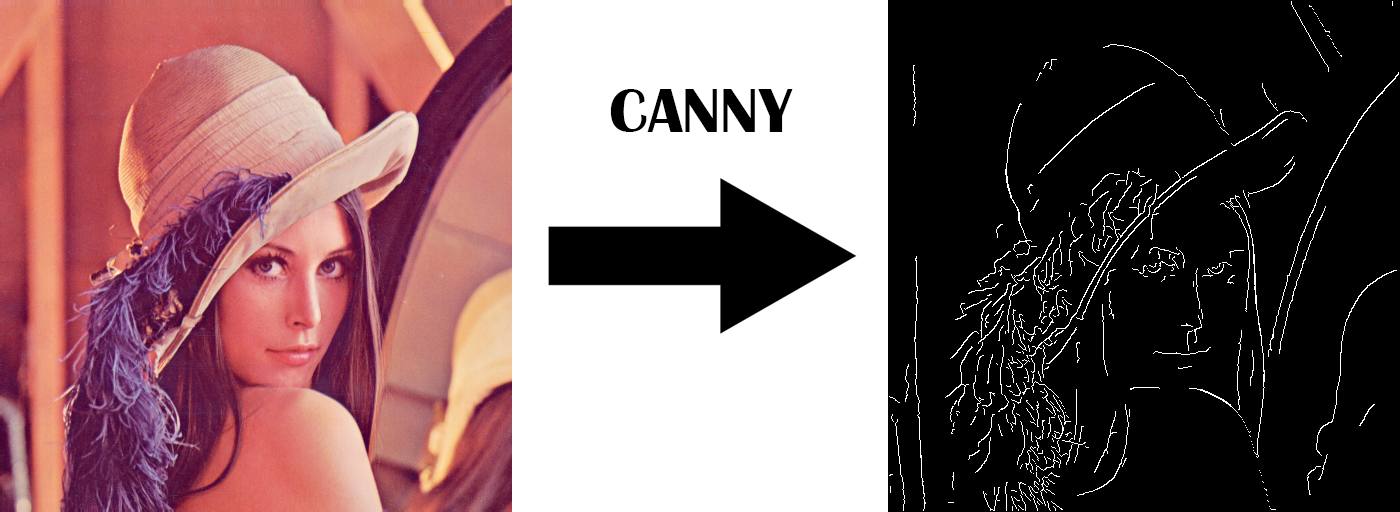
\includegraphics[width=\linewidth]{canny}
	\caption{Esempio di Canny Edge Detection}
\end{figure}
\chapter{Risultati ottenuti}

Sono state eseguite numerose prove che hanno \textit{confutato} quanto detto fino ad ora riguardo i vantaggi e problemi della parallelizzazione.\newline

\noindent In caso di immagine di \textit{dimensione troppo piccola}, i guadagni di performance vengono meno a causa dell'\textit{overhead} di creazione e comunicazione dei processi. L'esecuzione sequenziale ha sempre la meglio.

\begin{figure}[H]
	\centering
	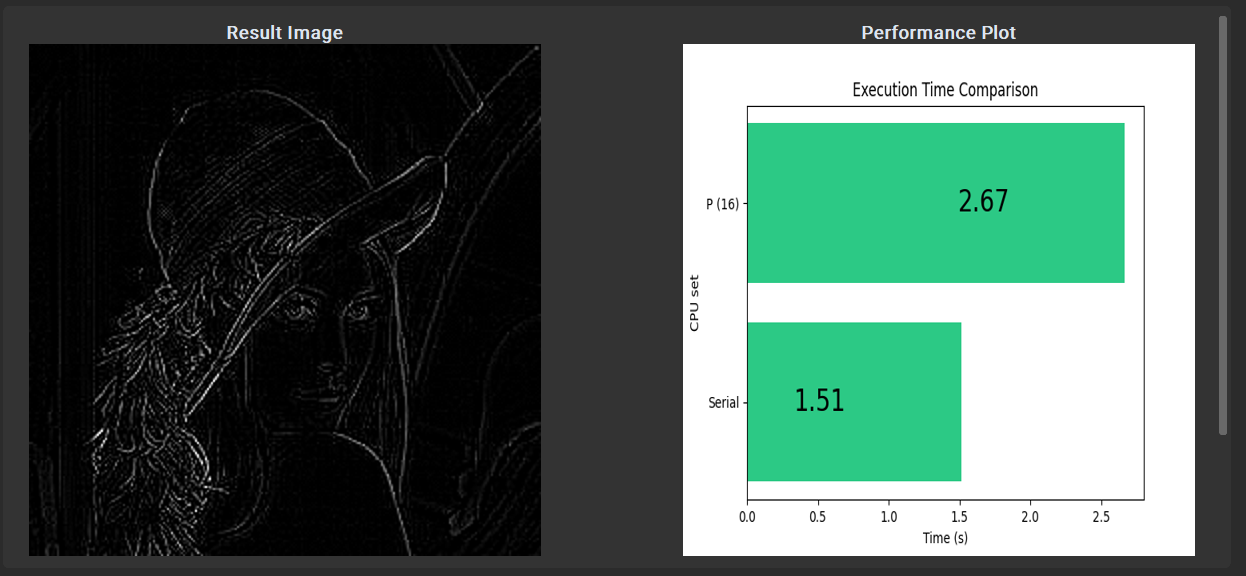
\includegraphics[width=\linewidth]{too-small}
	\caption{Esempio di parallelizzazione Lenna 256x256}
\end{figure}

\noindent In caso di immagine di \textit{dimensioni medie}, si hanno guadagni di performance con suddivisioni di piccolo taglio, tali guadagni vengono prima attenutati e successivamente persi man mano che aumentano le suddivisioni, sempre a causa dell'\textit{overhead} di creazione e comunicazione dei processi.

\begin{figure}[H]
	\centering
	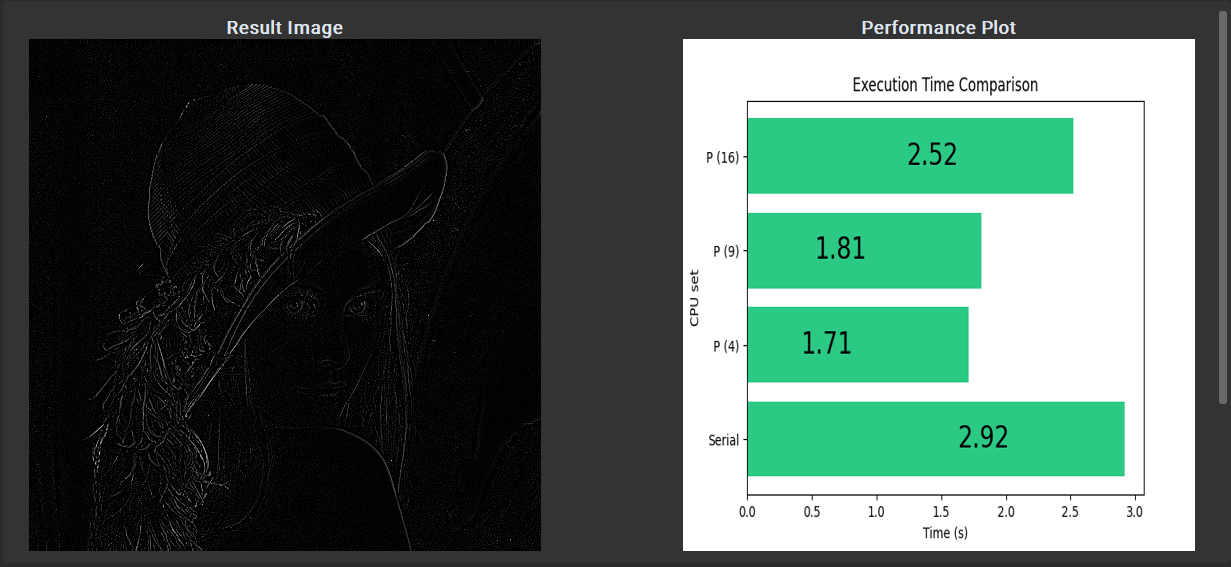
\includegraphics[width=\linewidth]{medium}
	\caption{Esempio di parallelizzazione Lenna 512x512}
\end{figure}


\noindent In caso di immagine di \textit{dimensioni grandi}, si hanno guadagni di performance evidenti. L'\textit{overhead} di creazione e comunicazione dei processi diventa meno trascurabile all'aumentare delle suddivisioni.

\begin{figure}[H]
	\centering
	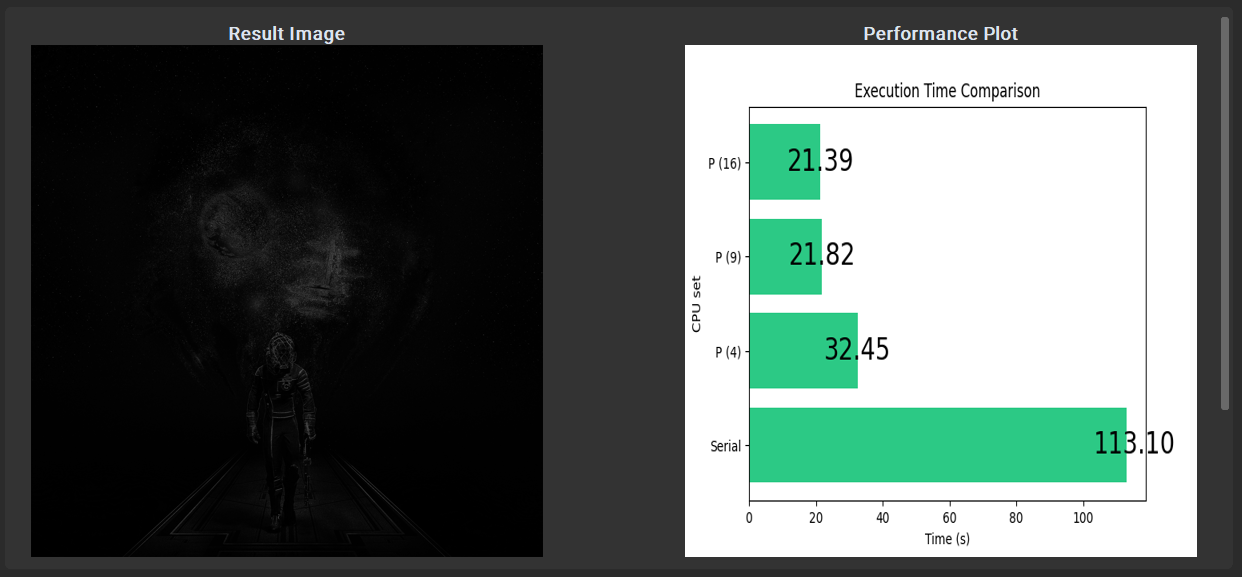
\includegraphics[width=\linewidth]{large}
	\caption{Esempio di parallelizzazione Prey 4000x4000}
\end{figure}


\noindent Infine, si è tentato un confronto fra la convoluzione implementata a mano e quella offerta dalla libreria \textit{SciPy}, il risultato è alquanto prevedibile in quanto tale libreria fa uso di implementazioni in C.
In tale configurazione il collo di bottiglia è rappresentato dalla tecnica di parallelizzazione di Python che degrada le performance offerte dal C.
\begin{figure}[H]
	\centering
	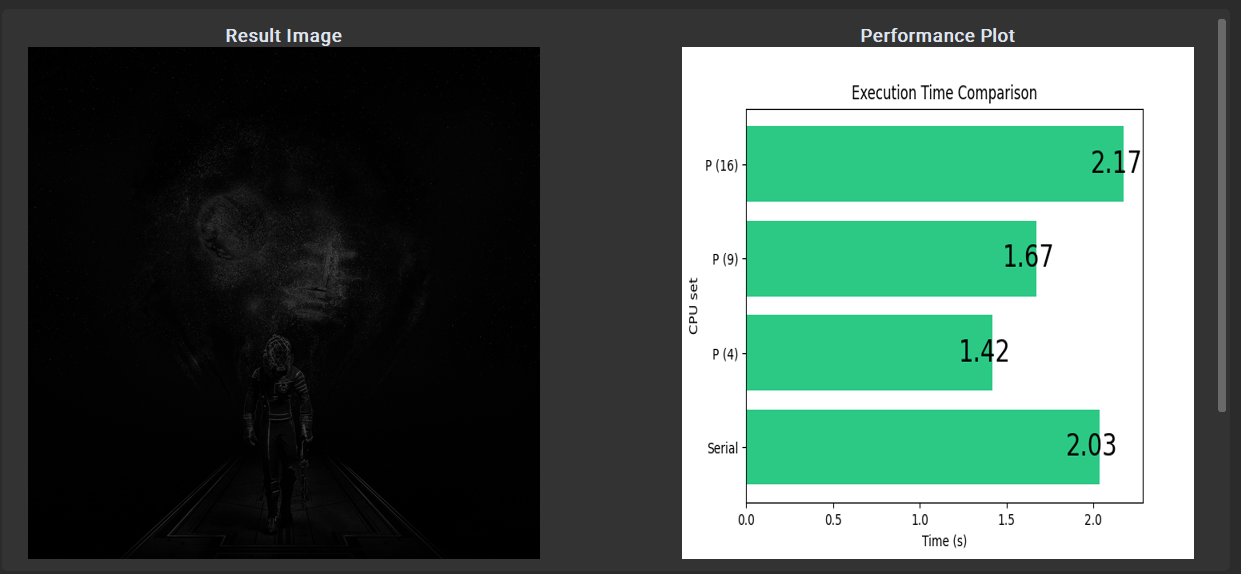
\includegraphics[width=\linewidth]{lib-conv}
	\caption{Esempio di parallelizzazione SciPy Prey 4000x4000}
\end{figure}



\begin{frontmatter}
\pagenumbering{arabic} \setcounter{page}{42}
\appendix
\chapter{Appendice}
\setcounter{secnumdepth}{0}
{\section{Codice Python}\label{appendix:image_subdivision}
	
\subsection{Suddivisione in linee}

{\begin{lstlisting}[language=Python, caption={Codice per la suddivisione in linee}, label={appendix:lines_subdivision}]
def _line_image_sub_divider(self) -> list[Image.Image]:
"""
Divide the image using lines.
:return: A list of the lines that the image is divided into.
"""
	tmp_image: Image.Image = self._target_image.copy()
	if self._target_cpu_core_set == 1:
		return [tmp_image]
	sub_images: list[Image.Image] = []
	line_width = tmp_image.width // self._target_cpu_core_set
	for i in range(self._target_cpu_core_set):
		left = i * line_width
		right = left + line_width
		sub_images.append(tmp_image.crop((left, 0, right, tmp_image.height)))
return sub_images
\end{lstlisting}}

{\begin{lstlisting}[language=Python, caption={Codice per l'unione delle linee}, label={appendix:lines_merge}]
def _merge_image_lines(self, lines: list[Image.Image]) -> Image.Image:
"""
Merge the lines of an image into one image.
:param lines: The lines to merge.
:return: The merged image.
"""
	if len(lines) == 1:
		return lines[0]
	tmp_image = Image.new("RGBA", self._target_image.size)
	line_width = tmp_image.width // self._target_cpu_core_set
	for i in range(self._target_cpu_core_set):
		left = i * line_width
		right = left + line_width
		tmp_image.paste(lines[i], (left, 0, right, tmp_image.height))
	return tmp_image
\end{lstlisting}}
\newpage
\subsection{Suddivisione in quadrati}

{\begin{lstlisting}[language=Python, caption={Codice per la suddivisione in quadrati}, label={appendix:square_subdivision}]
def _square_image_sub_divider(self) -> list[Image.Image]:
"""
Divide the image using squares.
:return: A list of the squares that the image is divided into.
"""
	tmp_image: Image.Image = self._target_image.copy()
	if self._target_cpu_core_set == 1:
		return [tmp_image]
	else:
		num_parts: int = int(self._target_cpu_core_set ** 0.5)
		square_size: int = tmp_image.width // num_parts
		sub_images: list[Image.Image] = []
		for row in range(num_parts):
			for column in range(num_parts):
				x_start: int = column * square_size
				y_start: int = row * square_size
				x_end: int = x_start + square_size
				y_end: int = y_start + square_size
				sub_images.append(tmp_image.crop((x_start, y_start, x_end, y_end)))
	return sub_images
\end{lstlisting}}

{\begin{lstlisting}[language=Python, caption={Codice per l'unione dei quadrati}, label={appendix:squares_merge}]
def _merge_image_squares(self, squares: list[Image.Image]) -> Image.Image:
"""
Merge the squares of an image into one image.
:param squares: The squares to merge.
:return: The merged image.
"""
	if len(squares) == 1:
		return squares[0]
	tmp_image = Image.new("RGBA", self._target_image.size)
	square_size: int = squares[0].width
	iterator: int = int(len(squares) ** 0.5)
	for row in range(iterator):
		for column in range(iterator):
			x_start: int = column * square_size
			y_start: int = row * square_size
			x_end: int = x_start + square_size
			y_end: int = y_start + square_size
			tmp_image.paste(squares[row * iterator + column], (x_start, y_start, x_end, y_end))
	return tmp_image
\end{lstlisting}}
\newpage
\subsection{Convoluzione}
{\begin{lstlisting}[language=Python, caption={Codice per la convoluzione}, label={appendix:convolution}]
def convolve_native(target_image: Image.Image, kernel: list[list[float]], gray_scale: bool = False) -> Image.Image:
"""
Convolves the target image with the given kernel.
:param target_image: The image to convolve.
:param kernel: The kernel to convolve with.
:param gray_scale: Whether to convert the image to grayscale before convolving.
:return: The convolved image.
"""
	img_type: str = "L" if gray_scale else "RGB"
	image_width, image_height = target_image.size
	kernel_size: int = len(kernel)
	padding: int = int(kernel_size / 2)
	result_image: Image.Image = Image.new(img_type, (image_width, image_height))
	target_image = target_image.convert(img_type)
	target_pixels = target_image.load()
	result_pixels = result_image.load()
	for y in range(image_height):
		for x in range(image_width):
			x_start: int = x - padding
			x_end: int = x + padding + 1
			y_start: int = y - padding
			y_end: int = y + padding + 1
			conv_pixel: list[float, float, float] | float = 0.0 if gray_scale else [0, 0, 0]
			iterator: int = 0
			for ky in range(y_start, y_end):
				for kx in range(x_start, x_end):
					px = max(0, min(kx, image_width - 1))
					py = max(0, min(ky, image_height - 1))
					pixel = target_pixels[px, py]
					kernel_value = kernel[int(iterator / kernel_size)][iterator % kernel_size]
					if gray_scale:
						conv_pixel += pixel * kernel_value
					else:
						conv_pixel[0] += pixel[0] * kernel_value
						conv_pixel[1] += pixel[1] * kernel_value
						conv_pixel[2] += pixel[2] * kernel_value
					iterator += 1
			normalized: tuple[int, int, int] | int
			if gray_scale:
				normalized: int = max(0, min(255, int(conv_pixel)))
			else:
				normalized: tuple[int, int, int] = (
					max(0, min(255, int(conv_pixel[0]))),
					max(0, min(255, int(conv_pixel[1]))),
					max(0, min(255, int(conv_pixel[2])))
				)
			result_pixels[x, y] = normalized
	return result_image
\end{lstlisting}}
\newpage
\subsection{Generazione Kernel di Gaussian}
{\begin{lstlisting}[language=Python, caption={Codice per la generazione di un kernel di Gauss}, label={appendix:gauss}]
def generate_gauss_kernel(kernel_size: int, sigma: int) -> list[list[float]]:
"""
Generates a Gaussian kernel of the given size and sigma.
:param kernel_size: The size of the kernel.
:param sigma: The sigma value.
:return: The generated kernel.
"""
	kernel = np.fromfunction(lambda x, y: (1 / (2 * np.pi * sigma ** 2)) * np.exp(
		-((x - (kernel_size - 1) / 2) ** 2 + (y - (kernel_size - 1) / 2) ** 2) / (2 * sigma ** 2)), (kernel_size, kernel_size))
	return (kernel / np.sum(kernel)).tolist()
\end{lstlisting}}

\subsection{Operatore Morfologico d'erosione}
{\begin{lstlisting}[language=Python, caption={Codice dell'operatore morfologico erosione}, label={appendix:erosion}]
def _erosion(target_image: Image.Image, structural_element: list[list[int]]) -> Image.Image:
"""
Applies the erosion operator to an RGB image.
:param target_image: The image to apply the operator to.
:param structural_element: The structural element to use.
:return: The eroded image.
"""
	width, height = target_image.size
	kernel_size: int = len(structural_element)
	target_image = target_image.convert("RGB")
	target_pixels = target_image.load()
	result_image = Image.new("RGB", (width, height))
	result_pixels = result_image.load()
	for y in range(height):
		for x in range(width):
			pixel_chs: list[int] = [255, 255, 255]
			for ky in range(kernel_size):
				for kx in range(kernel_size):
					px = x + kx - int(kernel_size / 2)
					py = y + ky - int(kernel_size / 2)
					if 0 <= px < width and 0 <= py < height:
						pixel_r, pixel_g, pixel_b = target_pixels[px, py]
						kernel_value = structural_element[ky][kx]
						pixel_chs[0] = min(pixel_chs[0], pixel_r - kernel_value)
						pixel_chs[1] = min(pixel_chs[1], pixel_g - kernel_value)
						pixel_chs[2] = min(pixel_chs[2], pixel_b - kernel_value)
			result_pixels[x, y] = (pixel_chs[0], pixel_chs[1], pixel_chs[2])
	return result_image
\end{lstlisting}}
\newpage
\subsection{Operatore Morfologico dilatazione}
{\begin{lstlisting}[language=Python, caption={Codice dell'operatore morfologico dilatazione}, label={appendix:dilation}]
def _dilation(target_image: Image.Image, structural_element: list[list[int]]) -> Image.Image:
"""
Applies the dilation operator to an RGB image.
:param target_image: The image to apply the operator to.
:param structural_element: The structural element to use.
:return: The dilated image.
"""
	width, height = target_image.size
	kernel_size: int = len(structural_element)
	target_image = target_image.convert("RGB")
	target_pixels = target_image.load()
	result_image = Image.new("RGB", (width, height))
	result_pixels = result_image.load()
	for y in range(height):
		for x in range(width):
			pixel_chs: list[int] = [0, 0, 0]
			for ky in range(kernel_size):
				for kx in range(kernel_size):
					px = x + kx - int(kernel_size / 2)
					py = y + ky - int(kernel_size / 2)
					if 0 <= px < width and 0 <= py < height:
						pixel_r, pixel_g, pixel_b = target_pixels[px, py]
						kernel_value = structural_element[ky][kx]
						pixel_chs[0] = max(pixel_chs[0], pixel_r + kernel_value)
						pixel_chs[1] = max(pixel_chs[1], pixel_g + kernel_value)
						pixel_chs[2] = max(pixel_chs[2], pixel_b + kernel_value)
			result_pixels[x, y] = (pixel_chs[0], pixel_chs[1], pixel_chs[2])
	return result_image
\end{lstlisting}}
\newpage
\subsection{Filtro di Media}
{\begin{lstlisting}[language=Python, caption={Codice del filtro di media}, label={appendix:mean}]
def mean_filter(target_image: Image.Image, filter_size: int) -> Image.Image:
"""
Applies the mean filter to an RGB image.
:param target_image: The image to apply the operator to.
:param filter_size: The size of the filter. By default it is 3.
:return: The filtered image.
"""	
	width, height = target_image.size
	half_size: int = int(filter_size / 2)
	target_image = target_image.convert("RGB")
	target_pixels = target_image.load()
	result_image = Image.new("RGB", (width, height))
	result_pixels = result_image.load()
	for x in range(width):
		for y in range(height):
			pixel_ch: list[int] = [0, 0, 0]
			count: int = 0
			for i in range(-half_size, half_size + 1):
				for j in range(-half_size, half_size + 1):
					nx = min(max(x + i, 0), width - 1)
					ny = min(max(y + j, 0), height - 1)
					pixel = target_pixels[nx, ny]
					pixel_ch[0] += pixel[0]
					pixel_ch[1] += pixel[1]
					pixel_ch[2] += pixel[2]
					count += 1
			result_pixels[x, y] = (int(pixel_ch[0] / count), int(pixel_ch[1] / count), int(pixel_ch[2] / count))
	return result_image
\end{lstlisting}}
\newpage
\subsection{Filtro Bilaterale}
{\begin{lstlisting}[language=Python, caption={Codice del filtro bilaterale}, label={appendix:bilateral}]
def bilateral_filter(target_image: Image.Image, diameter: int, sigma_color: int, sigma_space: int) -> Image.Image:
"""
Applies the bilateral filter to an RGB image.
:param target_image: The image to apply the operator to.
:param diameter: The diameter of the neighborhood.
:param sigma_color: The sigma color value. The greater the value, the colors farther to each other will start to get mixed
:param sigma_space: The sigma space value. The greater its value, the further pixels will mix together, given that their colors lie within the sigmaColor range.
:return: The filtered image.
"""
	def bilateral_filter_gaussian(dist: float, sigma_value: int) -> float:
		return (1 / (2 * math.pi * sigma_value ** 2)) * math.exp(-(dist ** 2) / (2 * sigma_value ** 2))
	width, height = target_image.size
	target_image = target_image.convert("RGB")
	target_pixels = target_image.load()
	result_image = Image.new("RGB", (width, height))
	result_pixels = result_image.load()
	for x in range(width):
		for y in range(height):
			r_acc, g_acc, b_acc = 0.0, 0.0, 0.0
			w_acc = 0.0
			for i in range(-diameter, diameter + 1):
				for j in range(-diameter, diameter + 1):
					nx = min(max(x + i, 0), width - 1)
					ny = min(max(y + j, 0), height - 1)
					pixel = target_pixels[nx, ny]
					spatial_dist = math.sqrt(i ** 2 + j ** 2)
					range_dist = math.sqrt((pixel[0] - target_pixels[x, y][0]) ** 2 +
						(pixel[1] - target_pixels[x, y][1]) ** 2 +
						(pixel[2] - target_pixels[x, y][2]) ** 2)

					weight = bilateral_filter_gaussian(spatial_dist, sigma_space) * bilateral_filter_gaussian(range_dist, sigma_color)
					r_acc += pixel[0] * weight
					g_acc += pixel[1] * weight
					b_acc += pixel[2] * weight
					w_acc += weight
			result_pixels[x, y] = (int(r_acc / w_acc), int(g_acc / w_acc), int(b_acc / w_acc))
	return result_image
\end{lstlisting}}
\newpage
\subsection{Canny Edge Detection}
{\begin{lstlisting}[language=Python, caption={Codice del filtro di Canny}, label={appendix:canny}]
def _non_maximal_supress(gradient_magnitude: np.ndarray, gradient_direction: np.ndarray) -> np.ndarray:
"""
Suppresses the non-maximal values in the given gradient magnitude array.
:param gradient_magnitude: The gradient magnitude array.
:param gradient_direction: The gradient direction array.
:return: The suppressed gradient magnitude array.
"""
	suppressed_magnitude = np.zeros_like(gradient_magnitude)
	angles = np.rad2deg(gradient_direction)
	angles[angles < 0] += 180
	for i in range(1, gradient_magnitude.shape[0] - 1):
		for j in range(1, gradient_magnitude.shape[1] - 1):
			direction = angles[i, j]
			if (0 <= direction < 22.5) or (157.5 <= direction <= 180):  # 0 degrees
				neighbors = [gradient_magnitude[i, j - 1], gradient_magnitude[i, j + 1]]
			elif 22.5 <= direction < 67.5:  # 45 degrees
				neighbors = [gradient_magnitude[i - 1, j - 1], gradient_magnitude[i + 1, j + 1]]
			elif 67.5 <= direction < 112.5:  # 90 degrees
				neighbors = [gradient_magnitude[i - 1, j], gradient_magnitude[i + 1, j]]
			else:  # 135 degrees
				neighbors = [gradient_magnitude[i - 1, j + 1], gradient_magnitude[i + 1, j - 1]]
			if gradient_magnitude[i, j] >= max(neighbors):
				suppressed_magnitude[i, j] = gradient_magnitude[i, j]
	return suppressed_magnitude

def _double_threshold(image_array: np.ndarray, low_threshold: int, high_threshold: int) -> np.ndarray:
"""
Filters the given image array with the given thresholds.
:param image_array: The image array.
:param low_threshold:
:param high_threshold:
:return: The filtered image array.
"""
	edge_map = np.zeros_like(image_array)
	edge_map[(image_array >= high_threshold)] = 255
	edge_map[(image_array >= low_threshold) & (image_array < high_threshold)] = 127
	return edge_map

def _link_edges(image_array: np.ndarray) -> np.ndarray:
"""
Links the edges of the given image array
:param image_array: The image array.
:return: Tge image array with the edges linked.
"""
	for i in range(1, image_array.shape[0] - 1):
		for j in range(1, image_array.shape[1] - 1):
			if image_array[i, j] == 127:
				if np.max(image_array[i - 1:i + 2, j - 1:j + 2]) == 255:
					image_array[i, j] = 255
				else:
					image_array[i, j] = 0
	return image_array


def canny_edge_detector(target_image: Image.Image, gauss_size: int, sigma: int, low_threshold: int,
high_threshold: int) -> Image.Image:
"""
Applies the canny edge detection algorithm to the given image.
:param target_image: The image to apply the canny algorithm to.
:param gauss_size: The size of the gaussian kernel.
:param sigma: The sigma value for the gaussian kernel.
:param low_threshold: The low threshold for the double thresholding.
:param high_threshold: The high threshold for the double thresholding.
:return: The image with the canny algorithm applied.
"""
	target_image = target_image.convert("L")
	# Phase 1 Smoothing applying gaussian kernel
	gauss_kernel = generate_gauss_kernel(gauss_size, sigma)
	gauss_image = convolve_native(target_image, gauss_kernel)
	# Phase 2 Finding the gradients
	sobel_x_array = np.array(convolve_native(gauss_image, convolution_kernels["edge_detection (sobel-x)"], True))
	sobel_y_array = np.array(convolve_native(gauss_image, convolution_kernels["edge_detection (sobel-y)"], True))
	gradient_magnitude = np.hypot(sobel_x_array, sobel_y_array)
	gradient_direction = np.arctan2(sobel_y_array, sobel_x_array)
	# Phase 3 Non-maximal supression
	supressed = _non_maximal_supress(gradient_magnitude, gradient_direction)
	# Phase 4 Double thresholding
	thresholded = _double_threshold(supressed, low_threshold, high_threshold)
	# Phase 5 Edge tracking by linking edges
	result_array = _link_edges(thresholded)
	return Image.fromarray(result_array.astype(np.uint8))
\end{lstlisting}}
\end{frontmatter}
\end{document}
